\documentclass[aspectratio=169,
hyperref={colorlinks,urlcolor=blue}
]{beamer}


%\usetheme{Pittsburgh}
\usetheme{default}
\usepackage{colortbl}%colored tables
%For using helvetica font:
\usepackage[scaled]{helvet}
\usepackage[T1]{fontenc}
\renewcommand\familydefault{\sfdefault}
\urlstyle{same} %sets the fonts for urls
\usepackage{pdfpages}
\usepackage{siunitx}
\usepackage{caption}
\usepackage{pifont}%for dings
\usepackage{pgfplots}%for 3d plotting
\pgfplotsset{compat = newest}
\usepackage{mathtools}%box in align env \Aboxed
\usepackage[american,smartlabels]{circuitikz}%for drawing circuits
\usepackage{multimedia}
\usepackage{animate}
\usepackage{xcolor}


\usetikzlibrary{arrows}
\usetikzlibrary {3d} 
\usetikzlibrary{decorations.markings, math}
\usetikzlibrary{intersections, pgfplots.fillbetween}
\usetikzlibrary {shapes.geometric} 


%\definecolor{myblue}{RGB}{5, 34, 150}
\definecolor{myblue2}{RGB}{5, 34, 150}
\definecolor{myblue}{RGB}{0,36,82}
\definecolor{myred}{RGB}{207, 2, 13}
\definecolor{mygreen}{RGB}{0, 158, 11}
\definecolor{myyellow}{RGB}{220,220,0}
\definecolor{qblue}{RGB}{0,36,82}
\definecolor{qgold}{RGB}{250,189,15}
\definecolor{qred}{RGB}{185,14,49}
\definecolor{cblue}{rgb}{0.13, 0.67, 0.8}
\definecolor{corange}{rgb}{0.8, 0.34, 0.0}
\definecolor{cpurple}{rgb}{0.54, 0.29, 0.42}

%%%%%%%%%%%% General settings
\setbeamercolor{frametitle}{fg=black}
\setbeamercolor{title}{fg=black}
\setbeamercolor{author}{fg=myblue2}

\beamertemplatenavigationsymbolsempty %no navigation controls at bottom of slides
%\setbeamertemplate{footline}[frame number]
\usefonttheme{professionalfonts} 
\setbeamerfont{title}{series=\bfseries,parent=structure}
\setbeamerfont{frametitle}{series=\bfseries,parent=structure}

%%%%%%%%%%%%Lists
\setbeamertemplate{itemize item}[circle] %{\color{myblue}$\circ$}
\setbeamertemplate{itemize subitem}{\color{myblue2}$\circ$}
\setbeamertemplate{itemize subsubitem}{\color{myblue2}$\cdot$}
\setbeamercolor{itemize item}{bg=myblue2,fg=myblue2}
\setbeamercolor{enumerate item}{bg=myblue2,fg=myblue2}
%%%%%%%%%%%%%%%%%%%%%%%%%%%%

%%%%%%%%%%%%Blocks
\setbeamertemplate{blocks}[rounded]
%Default block
\setbeamercolor{block title}{bg=myblue2, fg=white}
\setbeamercolor{block body}{bg=myblue2!10}
\setbeamerfont{block body}{size=\scriptsize}
\setbeamerfont{block title}{size=\scriptsize}
%Alert block
\setbeamercolor{block title alerted}{bg= myblue2, fg=white}
\setbeamercolor{block body alerted}{bg=myblue2!10}
\setbeamerfont{block body alerted}{size=\scriptsize}
\setbeamerfont{block title alerted}{size=\scriptsize}
%example block
\setbeamercolor{block title example}{bg=mygreen, fg=white}
\setbeamercolor{block body example}{bg=mygreen!10}
\setbeamerfont{block body example}{size=\scriptsize}
\setbeamerfont{block title example}{size=\scriptsize}
%%%%%%%%%%%%%%%%55


%%%%%%%%%%%%Figures and captions
\captionsetup{font=scriptsize,labelfont=scriptsize}
%\setbeamertemplate{caption}{\raggedright\insertcaption\par}
\newenvironment{capfig}[3]{\begin{figure}\includegraphics[width=#1\textwidth]{#2}\caption*{\textit{#3}}\end{figure}}{}

%\makeatother
%\setbeamertemplate{footline}
%{
%  \leavevmode%
%  \hbox{%
%  \begin{beamercolorbox}[wd=.4\paperwidth,ht=2.25ex,dp=1ex,center]{author in head/foot}%
%    \usebeamerfont{author in head/foot}\insertshortauthor
%  \end{beamercolorbox}%
%  \begin{beamercolorbox}[wd=.6\paperwidth,ht=2.25ex,dp=1ex,center]{title in head/foot}%
%    \usebeamerfont{title in head/foot}\insertshorttitle\hspace*{3em}
%    \insertframenumber{} / \inserttotalframenumber\hspace*{1ex}
%  \end{beamercolorbox}
%  }%
%  \vskip0pt%
%}
%\makeatletter

\makeatother
\setbeamertemplate{footline}
{
  \leavevmode%
  \hbox{%
\begin{beamercolorbox}[wd=.27\paperwidth,ht=2.25ex,dp=1ex,center]{author in head/foot}%
    \color{black}{\insertinstitute}
\end{beamercolorbox}
  \begin{beamercolorbox}[wd=.27\paperwidth,ht=2.25ex,dp=1ex,center]{author in head/foot}%
    \color{black}{\inserttitle}
  \end{beamercolorbox}%
  \begin{beamercolorbox}[wd=.27\paperwidth,ht=2.25ex,dp=1ex,center]{title in head/foot}%
    \color{black}{\insertshortauthor}
  \end{beamercolorbox}
  \begin{beamercolorbox}[wd=.27\paperwidth,ht=2.25ex,dp=1ex,center]{title in head/foot}%
    \hspace{.28\paperwidth}\color{black} \insertframenumber{} / \inserttotalframenumber\hspace*{1ex}
  \end{beamercolorbox}
  }%
  \vskip0pt%
}
\makeatletter

\setbeamertemplate{title page}
{
  \begin{tikzpicture}[remember picture,overlay]
    \def\barh{4}%15
  
    \draw[color=myblue2,line width=\barh] ([yshift=-0.5*\barh]current page.north west) -- ([yshift=-0.5*\barh,xshift=-0.67\paperwidth]current page.north east);
    \draw[color=myblue2,line width=\barh] ([yshift=-0.5*\barh,xshift=-0.67\paperwidth]current page.north east) -- ([yshift=-0.5*\barh,xshift=-0.34\paperwidth]current page.north east);
    \draw[color=myblue2,line width=\barh] ([yshift=-0.5*\barh,xshift=-0.34\paperwidth]current page.north east) -- ([yshift=-0.5*\barh]current page.north east); 
  
    \draw[color=myblue2,line width=\barh] ([yshift=0.5*\barh]current page.south west) -- ([yshift=0.5*\barh,xshift=-0.67\paperwidth]current page.south east);
    \draw[color=myblue2,line width=\barh] ([yshift=0.5*\barh,xshift=-0.67\paperwidth]current page.south east) -- ([yshift=0.5*\barh,xshift=-0.34\paperwidth]current page.south east);
    \draw[color=myblue2,line width=\barh] ([yshift=0.5*\barh,xshift=-0.34\paperwidth]current page.south east) -- ([yshift=0.5*\barh]current page.south east);
    %\node[left] at (current page.east) {
    %
\includegraphics[scale=0.1]{figures/coverpage}
    %};
  \end{tikzpicture}
  
  \usebeamerfont{title}\usebeamercolor[fg]{title}\inserttitle\par
  \usebeamerfont{subtitle}\usebeamercolor[fg]{subtitle}\insertsubtitle\par
  \vspace{2cm}
  \usebeamerfont{author}\usebeamercolor[fg]{author}\insertauthor\par
  \usebeamerfont{institute}\usebeamercolor[fg]{author}\insertinstitute\par
  \usebeamercolor[fg]{author}\par
  \usebeamercolor[fg]{titlegraphic}\inserttitlegraphic

} 

\setbeamertemplate{frametitle}{%
    \nointerlineskip%
        \par\hspace*{-\dimexpr0.5\paperwidth-0.5\textwidth}\textcolor{myblue2}{\rule{0.33\paperwidth}{6pt}}\textcolor{myblue2}{\rule{0.33\paperwidth}{6pt}}\textcolor{myblue2}{\rule{0.34\paperwidth}{6pt}} 
    \begin{beamercolorbox}[wd=\paperwidth,ht=0.75cm,dp=0.6ex]{frametitle}
        \hspace*{0.5cm}\strut\usebeamerfont{frametitle}\insertframetitle\strut
        %\hrule
    \end{beamercolorbox}%
    %%Line below:
%\par\hspace*{-\dimexpr0.5\paperwidth-0.5\textwidth}\textcolor{myblue}{\rule{\paperwidth}{0.4pt}}
     % <-- calculation of left margin width + rule
     %\textcolor{red}{\noindent\rule{\paperwidth}{2pt}}
}


%%%%%%%%%%%%Frame templates

%Slide with title
\newenvironment{titleframe}[1]
{\begin{frame}\frametitle{#1}\end{frame}}
{}

%Slide with title and itemize list:
\newenvironment{bulletframe}[1]
{\begin{frame}{#1} \itemize}
{\enditemize \end{frame}}

%Slide with two columns 50/50
\newenvironment{twocolframe}[3]
{\begin{frame}{#1}
 \begin{columns}[T]
 \column{0.5\textwidth}#2
 \column{0.5\textwidth}#3
 \end{columns}\end{frame}}{}

%Slide with two columns 60/40 <<<<<<<<<<<<<<<<<<<<<<  This one!
\newenvironment{twocolframesf}[3]
{\begin{frame}{#1}
 \begin{columns}[T]
 \column{0.6\textwidth}#2
 \column{0.4\textwidth}#3
 \end{columns}\end{frame}}{}
 
%Slide with two columns 70/30
\newenvironment{twocolframest}[3]
{\begin{frame}{#1}
 \begin{columns}[T] 
 \column{0.7\textwidth}#2
 \column{0.3\textwidth}#3
 \end{columns}\end{frame}}{} 
 
%Slide with two columns 40/60
\newenvironment{twocolframefs}[3]
{\begin{frame}{#1}
 \begin{columns}[T] 
 \column{0.4\textwidth}#2
 \column{0.6\textwidth}#3
 \end{columns}\end{frame}}{}
 
%Slide with two columns 70/30
\newenvironment{twocolframets}[3]
{\begin{frame}{#1}
 \begin{columns}[T] 
 \column{0.3\textwidth}#2
 \column{0.7\textwidth}#3
 \end{columns}\end{frame}}{} 

 
%Colloquium speaker (title, abstract, picture file, speaker name)
\newenvironment{colloquium}[5]
{
\begin{frame}{Colloquium: Friday 1:30pm in Stirling A}
\begin{columns}[T] 
 \column{0.8\textwidth}
 \textbf{#1}\\
 #2
 \column{0.2\textwidth}
 \capfig{#3}{#4}{#5}
 \end{columns}
\end{frame}
}
{} 

%%%%%%%%%%%%%Set Hyperref colors


\hypersetup{
  colorlinks=true,
  linkcolor=blue,    
  urlcolor=blue,     
  citecolor=blue      
}
%%%%%%%%%%%%%TOC bolding
\setbeamerfont{section in toc}{series=\bfseries}



%Frames:
% \twocolframesf 60/40 (fs, st, ts) 
% \titleframe
% bulletframe


%%%%%%%%%%%%%%%%%%%%%%%%%
%%%%%% START OF PRESENTATION %%%%%%
%%%%%%%%%%%%%%%%%%%%%%%%%
\title{Sources of Magnetic Fields}
\subject{Biot-Savart Law, Ampère's Law and Solenoids}
\subtitle{Building Models to Describe our World}


%%%%%%%%%%%%%%%%%%%%%%%%%%%%%%
%%%%%%%%%%%%%%%%%%%%%



\begin{document}

%%%%%%%%%%%%%%%%%%%%%%%%%
%%%%%% Title slide %%%%%%
%%%%%%%%%%%%%%%%%%%%%%%%%
\chaptertitle{Sources of Magnetic FIelds}
\begin{frame}
\titlepage
\thispagestyle{empty}

\begin{textblock*}{5cm}(11cm,4cm)
    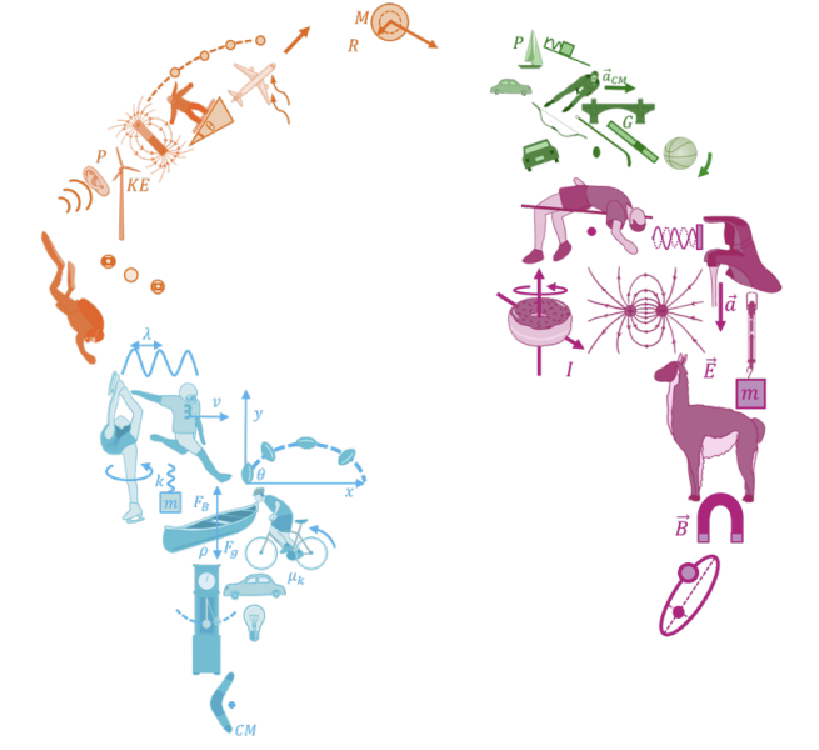
\includegraphics[width=4cm]{figures/BMDW/logo}
\end{textblock*}

\end{frame}

%%%%%%%%%%%%%TOC
\twocolframe{Outline}
  {\tableofcontents[sections={1}, subsectionstyle=show/show]\thispagestyle{empty}}
  {\tableofcontents[sections={2,3}, subsectionstyle=show/show]}
%%%%%%%%%%%%%%%%%%%%%%%%%







%%%%%%%%%%%%%%%%%%%%%%%%%%%%%%%%
\section{Biot-Savart Law}
\label{sec:biorsavartlaw}
\title{Biot-Savart Law}


%%%%%%%%%%%%%%%%%%%%%%%%%
\begin{frame}
\titlepage
\thispagestyle{empty}
\end{frame}

%%%%%%%%%%%%%%%%%%%%%%%%%%




\subsection{Review: calculating the electric field}
\label{subsec:reviewcalulatingtheelectricfield}
\begin{frame}{Review: Calculating the electric field}

Three ways to determine the electric field:
\begin{enumerate}
\item Model a charge distribution as the sum of point charges, $dq$:
\begin{align*}
E = \int dE=\int k\frac{dq}{r^2}
\end{align*}
\item Exploit symmetry and use Gauss' Law:
\begin{align*}
\oint \vec E \cdot d\vec A= \frac{Q}{\epsilon_0}
\end{align*}
\item Build from common charge distributions (e.g. model a plane as many lines of charge):
\begin{align*}
E=\frac{\lambda}{2\pi\epsilon_0 r}
\end{align*}
\end{enumerate}
\end{frame}

%%%%%%%%%%%%%%%%%%%%%%%%%%%%%%



%%%%%%%%%%%%%%%%%%%%%%%%%%%%%%
\subsection{Formula}
\label{subsec:bsformula}
\twocolframesf{The Biot-Savart Law}
{
A small section of wire, $d\vec l$, carrying current, $I$, will create a magnetic field, $d\vec B$, given by:
\begin{align*}
d\vec B = \frac{\mu_0I}{4\pi}\frac{d\vec l\times \hat r}{r^2}
\end{align*}
\begin{itemize}
\item $d\vec l$: the small segment (along wire, in direction of $I$).
\item $\vec r$: a vector \textbf{from the segment} to where we want to calculate the field.
\item $r$: the magnitude of $\vec r$.
\item $\hat r$: unit vector in direction of $\vec r$.  
\end{itemize}
}
{
\centering
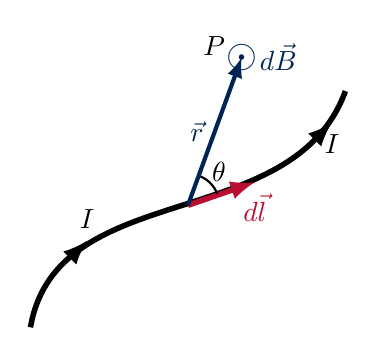
\begin{tikzpicture}[scale=1]

\coordinate (a) at (0.62,1);
\coordinate (b) at (3.73,2.5);
\coordinate (c) at (2,1.55);
\coordinate (P) at ($(c)+(70:2)$);
%\fill (c) circle(3pt);

\draw[line width=2] (0,0) [out=80, in=250] to (4,3);
\draw[-latex, line width=2] (a) -- +(0.1,0.1) node[above]{$I$};
\draw[-latex, line width=2] (b) -- +(0.1,0.1) node[below]{$I$};
\draw[-latex, line width=2, color=qred] (c) -- +(19:0.9) node[below]{$d\vec l$};

\draw[line width=0.8] ($(c)+(70:0.4)$) arc (70:21:0.4)node[midway,above=4pt, right=-3pt]{$\theta$};

\draw[-latex, line width=1.5, color=qblue] (c) -- (P)node[midway,left]{$\vec r$};

\node[left=10pt,above=-3pt] at (P) {$P$};
\node[color=qblue] at (P) {\Large $\odot$};
\node[right=3pt, color=qblue] at (P) {$d\vec B$};
\end{tikzpicture}
\captionof*{figure}{\textit{Using the Biot-Savart law to determine the magnetic field at point $P$ due to the wire carrying current, $I$.}}

}

%%%%%%%%%%%%%%%%%%%%%%%%%%%%%%



%%%%%%%%%%%%%%%%%%%%%%%%%%%%%%
\subsection{The unit vector}
\label{subsec:theunitvector}
\begin{frame}{The unit vector}
\begin{itemize}
\item In practice, it is not always convenient to first calculate a vector, $\vec r$, and then a unit vector in that direction. Can use $\vec r$  directly in the Biot-Savart law:
\begin{align*}
d\vec B = \frac{\mu_0I}{4\pi}\frac{d\vec l\times \textcolor{qred}{\hat r}}{r^{\textcolor{qred}{2}}}
=\frac{\mu_0I}{4\pi}\frac{d\vec l\times \textcolor{qred}{\frac{\vec r}{r}}}{r^{\textcolor{qred}{2}}}
 = \frac{\mu_0I}{4\pi}\frac{d\vec l\times \textcolor{qred}{\vec r}}{r^{\textcolor{qred}{3}}} 
\end{align*}
\end{itemize}
\end{frame}


%%%%%%%%%%%%%%%%%%%%%%%%%%%%%%
\subsection{Magnetic field from a finite straight wire}
\label{subsec:magneticfieldfromafinitestraightwire}
\twocolframesf{Magnetic field from a straight wire of length $L$}
{
\begin{enumerate}
\item<1-> Make a good diagram.
\item<2-> Choose $d\vec l$.
\item<3-> Determine $d\vec l \times \vec r$:
\only<3>{
}
\only<4>{
\begin{align*}
d\vec l \times \vec r &= (dl \hat y) \times (r\cos\theta\hat x-r\sin\theta\hat y)
\end{align*}
}
\only<5>{
\begin{align*}
d\vec l \times \vec r &= (dl \hat y) \times (r\cos\theta\hat x-r\sin\theta\hat y)\\
&=dlr\cos\theta (\hat y\times \hat x) - dlr\sin\theta(\hat y \times \hat y)
\end{align*}
}
\only<6>{
\begin{align*}
d\vec l \times \vec r &= (dl \hat y) \times (r\cos\theta\hat x-r\sin\theta\hat y)\\
&=dlr\cos\theta \cancelto{(-\hat z)}{(\hat y\times \hat x)} - dlr\sin\theta\cancelto{0}{(\hat y \times \hat y)}
\end{align*}
}
\only<7>{
\begin{align*}
d\vec l \times \vec r &= (dl \hat y) \times (r\cos\theta\hat x-r\sin\theta\hat y)\\
&=dlr\cos\theta \cancelto{(-\hat z)}{(\hat y\times \hat x)} - dlr\sin\theta\cancelto{0}{(\hat y \times \hat y)}\\
&=-dlr\cos\theta\hat z
\end{align*}
}
\only<8->{
\begin{align*}
d\vec l \times \vec r =-r\cos\theta dl \hat z
\end{align*}
}
\item<8-> Determine $d\vec B$:
\only<9->{
\begin{align*}
d\vec B = \frac{\mu_0I}{4\pi}\frac{d\vec l\times \vec r}{r^3} =-\frac{\mu_0I}{4\pi}\frac{\cos\theta}{r^2}dl\hat z
\end{align*}

}

\end{enumerate}
}
{
\vspace{-0.25cm}
\centering
\begin{tikzpicture}[scale=1]
\def\L{5}
\def\D{3}
\def\dl{0.75}

\coordinate (P) at (\D,0);
\coordinate (PL) at (0,0.25*\L);


%Set up:
\draw[line width =3] (0,-\L/2) -- (0,\L/2);
\fill (P) circle(2pt);
\node[above=10pt,right=2pt] at (P) {$P$}; 
\draw[-latex] (0,0) -- ($(P)+(1.5\D,0)$) node[below]{$x$};
\draw[-latex,line width =3] (0,-0.5*\L) -- (0,-0.25*\L) node[right]{$I$};
\draw[-latex] (0,-0.6*\L) -- (0,0.6*\L) node[left]{$y$};
\draw[latex-latex] (-0.15*\L,-0.5*\L) -- (-0.15*\L,0.5*\L) node[midway,left]{$L$};
\draw[latex-latex] (0,-0.02*\L) -- (\D,-0.02*\L) node[midway, below] {$D$};


%construction
\only<2->{
\draw[-latex,color=qred,line width =3] ($ (PL)+(0,-0.5*\dl) $) -- +(0,\dl)node[midway,left]{$d\vec l$};
\draw[-latex, line width=1.5pt] (PL) -- (P) node[midway,above]{$\vec r$};
\begin{scope}
\clip (PL) -- (P) -- (0,0) --(PL);
\draw ($(P)+(-0.4*\D,0)$) arc(180:90:0.4*\D);
\end{scope}
\node[above] at (0.5*\D,0) {$\theta$};
}
\only<9->{%dB
\node[right=-5pt,color=qblue!80] at (P) {\huge $\times$};
\node[right=3pt, below=3pt,color=qblue!80] at (P) {$d\vec B$};
}
\end{tikzpicture}
\captionof*{figure}{\textit{Using the Biot-Savart law to determine the magnetic field at point $P$ due to the wire carrying current, $I$.}}
}

%%%%%%%%%%%%%%%%%%%%%%%%%%%%%%
\twocolframesf{Magnetic field from a straight wire of length $L$}
{
\begin{enumerate}
\setcounter{enumi}{3}
\item<1-> Determine $d\vec B$:
\begin{align*}
d\vec B =-\frac{\mu_0I}{4\pi}\cos\theta\frac{1}{r^2}dl\hat z
\end{align*}
\item<1-> Need to choose variable of integration ($dy$, $d\theta$) to integrate.
\only<3-5>{
\begin{itemize}
\item[$\rightarrow$]Choose $d\theta$:
\only<4-5>{
\begin{align*}
r &= \frac{D}{\cos\theta}\quad&\rightarrow & \quad &\therefore\quad &\frac{1}{r^2}&=&\frac{\cos^2}{D^2}\\
l &= D\tan\theta\quad&\rightarrow&\quad &\therefore\quad&dl&=&\frac{D}{\cos^2\theta}d\theta\\
\end{align*}
}
\only<5>{
\vspace{-1cm}
\begin{align*}
\therefore d\vec B =-\frac{\mu_0I}{4\pi}\cos\theta \frac{\cos^2\theta}{D^2}\frac{D}{\cos^2\theta}d\theta\hat z = -\frac{\mu_0I}{4\pi}\frac{\cos\theta}{D}d\theta\hat z
\end{align*}
}
\end{itemize}
}
\end{enumerate}
}
{
\vspace{-0.25cm}
\centering
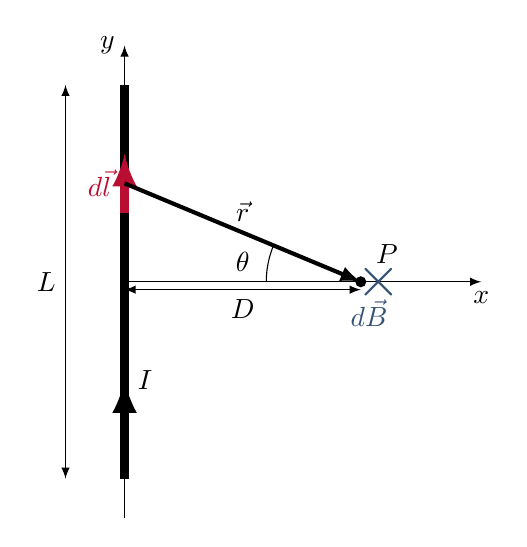
\begin{tikzpicture}[scale=1]
\def\L{5}
\def\D{3}
\def\dl{0.75}

\coordinate (P) at (\D,0);
\coordinate (PL) at (0,0.25*\L);


%Set up:
\draw[line width =3] (0,-\L/2) -- (0,\L/2);
\fill (P) circle(2pt);
\node[above=10pt,right=2pt] at (P) {$P$}; 
\draw[-latex] (0,0) -- ($(P)+(1.5\D,0)$) node[below]{$x$};
\draw[-latex,line width =3] (0,-0.5*\L) -- (0,-0.25*\L) node[right]{$I$};
\draw[-latex] (0,-0.6*\L) -- (0,0.6*\L) node[left]{$y$};
\draw[latex-latex] (-0.15*\L,-0.5*\L) -- (-0.15*\L,0.5*\L) node[midway,left]{$L$};
\draw[latex-latex] (0,-0.02*\L) -- (\D,-0.02*\L) node[midway, below] {$D$};

\draw[-latex,color=qred,line width =3] ($ (PL)+(0,-0.5*\dl) $) -- +(0,\dl)node[midway,left]{$d\vec l$};
\draw[-latex, line width=1.5pt] (PL) -- (P) node[midway,above]{$\vec r$};
\begin{scope}
\clip (PL) -- (P) -- (0,0) --(PL);
\draw ($(P)+(-0.4*\D,0)$) arc(180:90:0.4*\D);
\end{scope}
\node[above] at (0.5*\D,0) {$\theta$};

\node[right=-5pt,color=qblue!80] at (P) {\huge $\times$};
\node[right=3pt, below=3pt,color=qblue!80] at (P) {$d\vec B$};

\end{tikzpicture}
\captionof*{figure}{\textit{Using the Biot-Savart law to determine the magnetic field at point $P$ due to the wire carrying current, $I$.}}
}


%%%%%%%%%%%%%%%%%%%%%%%%%%%%%%
\twocolframesf{Magnetic field from a straight wire of length $L$}
{
\begin{enumerate}
\setcounter{enumi}{5}
\item<1-> Do the integral:
\only<1>{
\begin{align*}
\vec B &= \int d\vec B =-\frac{\mu_0I}{4\pi D}\int_{\textcolor{qred}{-\theta_0}}^{\textcolor{qred}{+\theta_0}}\cos\theta d\theta\hat z
\end{align*}
}
\only<2>{
\begin{align*}
\vec B &= \int d\vec B =-\frac{\mu_0I}{4\pi D}\int_{\textcolor{qred}{-\theta_0}}^{\textcolor{qred}{+\theta_0}}\cos\theta d\theta\hat z\\
&=-\frac{\mu_0I}{4\pi D}\left[\sin\theta\right]_{-\theta_0}^{\theta_0}\hat z=-\frac{\mu_0I}{2\pi D}\sin\theta_0\hat z
\end{align*}
}
\only<3>{
\begin{align*}
\vec B &= \int d\vec B =-\frac{\mu_0I}{4\pi D}\int_{\textcolor{qred}{-\theta_0}}^{\textcolor{qred}{+\theta_0}}\cos\theta d\theta\hat z\\
&=-\frac{\mu_0I}{4\pi D}\left[\sin\theta\right]_{-\theta_0}^{\theta_0}\hat z=-\frac{\mu_0I}{2\pi D}\sin\theta_0\hat z\\
\therefore \vec B&=-\frac{\mu_0I}{2\pi D} \frac{L/2}{\sqrt{\left(L/2\right)^2+D^2}}{}  \hat z\\
\end{align*}
}
\end{enumerate}
}
{
\vspace{-0.25cm}
\centering
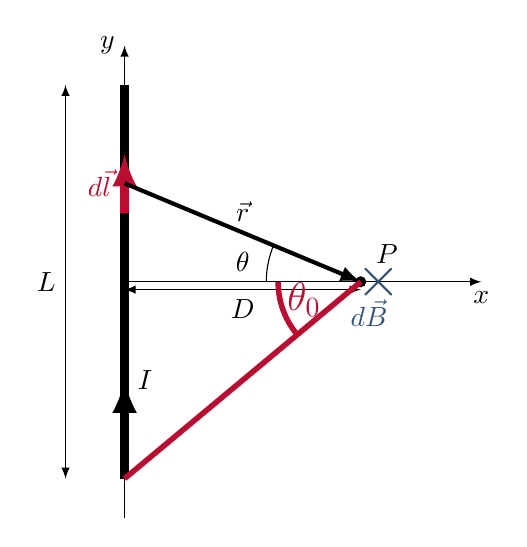
\begin{tikzpicture}[scale=1]
\def\L{5}
\def\D{3}
\def\dl{0.75}

\coordinate (P) at (\D,0);
\coordinate (PL) at (0,0.25*\L);


%Set up:
\draw[line width =3] (0,-\L/2) -- (0,\L/2);
\fill (P) circle(2pt);
\node[above=10pt,right=2pt] at (P) {$P$}; 
\draw[-latex] (0,0) -- ($(P)+(1.5\D,0)$) node[below]{$x$};
\draw[-latex,line width =3] (0,-0.5*\L) -- (0,-0.25*\L) node[right]{$I$};
\draw[-latex] (0,-0.6*\L) -- (0,0.6*\L) node[left]{$y$};
\draw[latex-latex] (-0.15*\L,-0.5*\L) -- (-0.15*\L,0.5*\L) node[midway,left]{$L$};
\draw[latex-latex] (0,-0.02*\L) -- (\D,-0.02*\L) node[midway, below] {$D$};

\draw[-latex,color=qred,line width =3] ($ (PL)+(0,-0.5*\dl) $) -- +(0,\dl)node[midway,left]{$d\vec l$};
\draw[-latex, line width=1.5pt] (PL) -- (P) node[midway,above]{$\vec r$};
\begin{scope}
\clip (PL) -- (P) -- (0,0) --(PL);
\draw ($(P)+(-0.4*\D,0)$) arc(180:90:0.4*\D);
\end{scope}
\node[above] at (0.5*\D,0) {$\theta$};

\node[right=-5pt,color=qblue!80] at (P) {\huge $\times$};
\node[right=3pt, below=3pt,color=qblue!80] at (P) {$d\vec B$};

%theta_0
\draw[line width =2pt,color=qred] (P) -- (0,-\L/2);
\begin{scope}
\clip (0,-\L/2)-- (P) -- (0,0) --(0,-\L/2);
\draw[line width =2pt,color=qred] ($(P)+(-0.35*\D,0)$) arc(180:270:0.35*\D);
\end{scope}
\node[below=-3pt,color=qred] at (0.76*\D,0) {\Large $\theta_0$};

\end{tikzpicture}
\captionof*{figure}{\textit{Using the Biot-Savart law to determine the magnetic field at point $P$ due to the wire carrying current, $I$.}}
}

%%%%%%%%%%%%%%%%%%%%%%%%%%%%%%




%%%%%%%%%%%%%%%%%%%%%%%%%%%%%%
\subsection{Magnetic field from an infinitely-long wire}
\label{subsec:magneticfieldfromaninfinitelylongwire}
\twocolframesf{Magnetic field from an infinitely-long wire}
{
\capfig{0.25}{figures/Bsource/axishand}{Right hand rule for axial vectors, used with thumb parallel to current.}
\begin{itemize}
\item The field lines are concentric with the wire (right hand rule for axial vectors).
\item The magnitude of the field at point, $P$, a distance, $r$, from the wire is:
\begin{align*}
B=\frac{\mu_0 I}{2\pi r}
\end{align*}
\end{itemize}
}
{
\centering
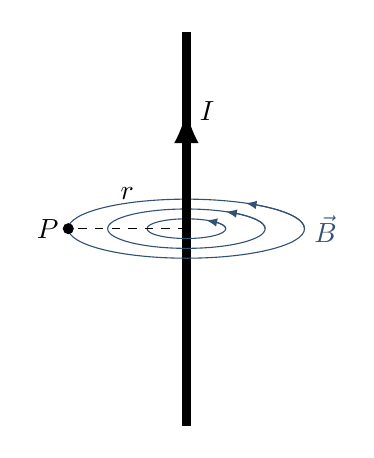
\begin{tikzpicture}[scale=1]
\def\L{5}
\def\D{1}

\draw[line width =3] (0,-\L/2) -- (0,\L/2);

\draw[color=qblue!80] (0,0) circle [x radius=0.5*\D, y radius=0.5*\D/4];
\draw[-latex, color=qblue!80] (0.5*\D,0) arc(0:60:{0.5*\D} and {0.5*\D/4});
\draw[color=qblue!80] (0,0) circle [x radius=\D, y radius=\D/4];
\draw[-latex, color=qblue!80] (1.0*\D,0) arc(0:60:{1.0*\D} and {1.0*\D/4});
\draw[color=qblue!80] (0,0) circle [x radius=1.5*\D, y radius=1.5*\D/4];
\draw[-latex, color=qblue!80] (1.5*\D,0) arc(0:60:{1.5*\D} and {1.5*\D/4});
\node[right, color=qblue!80] at (1.5*\D,0) {$\vec B$};
\draw[dashed] (0,0) -- (-1.5*\D,0) node[midway,above=7pt] {$r$};
\fill (-1.5*\D,0) circle(2pt);
\node[left] at (-1.5*\D,0) {$P$};
\draw[-latex,line width =3] (0,0) -- (0,0.3*\L) node[right]{$I$};

\end{tikzpicture}
\captionof*{figure}{\textit{Magnetic field forms concentric circles around the wire.}}
}

%%%%%%%%%%%%%%%%%%%%%%%%%%%%%%
\begin{bulletframe}{Force between 2 wires}
\item A wire carrying current produces a magnetic field:
\begin{align*}
B=\frac{\mu_0 I}{2\pi r}
\end{align*}
\item A wire carrying current in a magnetic field feels a force:
\begin{align*}
\vec F = I \vec l \times \vec B
\end{align*}
\item[$\rightarrow$] Two wires next to each other both carrying current must exert forces on each other!
\end{bulletframe}

%%%%%%%%%%%%%%%%%%%%%%%%%%%%%%



%%%%%%%%%%%%%%%%%%%%%%%%%%%%%%


%%%%%%%%%%%%%%%%%%%%%%%%%%%%%%
\subsection{Force between two wires}
\label{subsec:forcebetweentwowires}
\twocolframesf{Force between two wires}
{
\begin{itemize}
\item The field from wire 1:
\begin{align*}
B_1=\frac{\mu_0 I_1}{2\pi d}
\end{align*}
\item <2->The force on wire 2:
\begin{align*}
F_2 = I_2 L B_1 = \frac{\mu_0 I_1I_2 L}{2\pi d}
\end{align*}
\item<3-> Is the force on wire 1 from wire 2 the same?
\item<4->[$\rightarrow$] Newton's Third Law...
\end{itemize}
}
{
\centering
\begin{tikzpicture}[scale=1]
\def\L{5}
\def\D{2}

\draw[line width =3] (-\D/2,-\L/2) -- (-\D/2,\L/2);
\draw[line width =3] (\D/2,-\L/2) -- (\D/2,\L/2);
\draw[-latex,line width =3] (-\D/2,0) -- (-\D/2,0.3*\L) node[right]{$I_1$};
\draw[-latex,line width =3] (\D/2,0) -- (\D/2,0.3*\L) node[right]{$I_2$};


\draw[color=qblue!80] (-\D/2,0) circle [x radius=\D, y radius=\D/4];
\draw[-latex, color=qblue!80] (1.0*\D-\D/2,0) arc(0:60:{1.0*\D} and {1.0*\D/4}) node [above] {$\vec  B_1$};
\draw[latex-latex] (-\D/2,-0.25*\L) -- (\D/2,-0.25*\L) node[midway,below] {$d$} ;
%force vectors
\only<2->{
\draw[-latex,color=qred, line width =1.5pt] (\D/2,0) -- (0,0) node[below]{$\vec F$};
}
\only<4->{
\draw[color=qblue!80] (\D/2,0) circle [x radius=\D, y radius=\D/4];
\draw[-latex, color=qblue!80] (1.0*\D+\D/2,0) arc(0:60:{1.0*\D} and {1.0*\D/4}) node [above] {$\vec  B_2$};

\draw[-latex,color=qred, line width =1.5pt] (-\D/2,0) -- (0,0);
}
\end{tikzpicture}
\captionof*{figure}{\textit{Force between two wires}}
}



%%%%%%%%%%%%%%%%%%%%%%%%







%%%%%%%%%%%%%%%%%%%%%%%%




%%%%%%%%%%%%%%%%%%%%%%%%%%%%%%



%%%%%%%%%%%%%%%%%%%%%%%%%%%%%%
\twocolframesf{Field from a loop}
{
\begin{itemize}
\item Think of each section of the wire as a small straight wire.
\item The field looks like that from a bar magnet.
\end{itemize}
\begin{center}

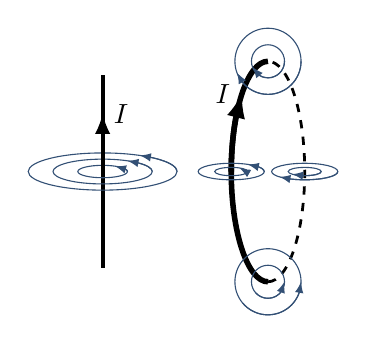
\begin{tikzpicture}[scale=0.7]
\def\R{2}
\def\Rt{\R/3}
\def\sc{0.5}
\def\D{0.6}

%straight wire (like a sub figure)
\begin{scope}[scale=\sc,rotate=0,shift={(-3*\R,0)}]
\def\L{7}
\def\D{1.8}
\draw[line width =1.5pt] (0,-\L/2) -- (0,\L/2);
\draw[color=qblue!80] (0,0) circle [x radius=0.5*\D, y radius=0.5*\D/4];
\draw[-latex, color=qblue!80] (0.5*\D,0) arc(0:60:{0.5*\D} and {0.5*\D/4});
\draw[color=qblue!80] (0,0) circle [x radius=\D, y radius=\D/4];
\draw[-latex, color=qblue!80] (1.0*\D,0) arc(0:60:{1.0*\D} and {1.0*\D/4});
\draw[color=qblue!80] (0,0) circle [x radius=1.5*\D, y radius=1.5*\D/4];
\draw[-latex, color=qblue!80] (1.5*\D,0) arc(0:60:{1.5*\D} and {1.5*\D/4});
\draw[-latex,line width =1.5] (0,0) -- (0,0.3*\L) node[right]{$I$};
\end{scope}

%big loop
\draw[line width =2pt] (0,-\R) arc(270:90:{\Rt} and {\R});
\draw[line width =1pt, dashed] (0,-\R) arc(-90:90:{\Rt} and {\R});
\draw[line width =2pt,-latex] (-\Rt,0) arc(180:135:{\Rt} and \R) node[left] {$I$};
%fields
%fields around big loop
\begin{scope}[scale=1,rotate=0,shift={(-\Rt,0)}]
\draw[color=qblue!80] (0,0) circle [x radius=0.5*\D, y radius=0.5*\D/4];
\draw[-latex, color=qblue!80] (0.5*\D,0) arc(0:60:{0.5*\D} and {0.5*\D/4});
\draw[color=qblue!80] (0,0) circle [x radius=\D, y radius=\D/4];
\draw[-latex, color=qblue!80] (1.0*\D,0) arc(0:60:{1.0*\D} and {1.0*\D/4});
%\draw[color=qblue!80] (0,0) circle [x radius=1.5*\D, y radius=1.5*\D/4];
%\draw[-latex, color=qblue!80] (1.5*\D,0) arc(0:60:{1.5*\D} and {1.5*\D/4});
\end{scope}

\begin{scope}[scale=1,shift={(\Rt,0)}]
\draw[color=qblue!80] (0,0) circle [x radius=0.5*\D, y radius=0.5*\D/4];
\draw[-latex, color=qblue!80] (0.5*\D,0) arc(0:-140:{0.5*\D} and {0.5*\D/4});
\draw[color=qblue!80] (0,0) circle [x radius=\D, y radius=\D/4];
\draw[-latex, color=qblue!80] (1.0*\D,0) arc(0:-140:{1.0*\D} and {1.0*\D/4});
%\draw[color=qblue!80] (0,0) circle [x radius=1.5*\D, y radius=1.5*\D/4];
%\draw[-latex, color=qblue!80] (1.5*\D,0) arc(0:60:{1.5*\D} and {1.5*\D/4});
\end{scope}

\begin{scope}[scale=1,shift={(0,\R)}]
\draw[color=qblue!80] (0,0) circle (0.5*\D);
\draw[-latex, color=qblue!80] (0.5*\D,0) arc(0:-160:{0.5*\D} and {0.5*\D});
\draw[color=qblue!80] (0,0) circle (\D);
\draw[-latex, color=qblue!80] (1.0*\D,0) arc(0:-160:{1.0*\D} and {1.0*\D});
\end{scope}

\begin{scope}[scale=1,shift={(0,-\R)}]
\draw[color=qblue!80] (0,0) circle (0.5*\D);
\draw[latex-, color=qblue!80] (0.5*\D,0) arc(0:-140:{0.5*\D} and {0.5*\D});
\draw[color=qblue!80] (0,0) circle (\D);
\draw[latex-, color=qblue!80] (1.0*\D,0) arc(0:-140:{1.0*\D} and {1.0*\D});
\end{scope}

\end{tikzpicture}
\captionof*{figure}{\textit{From the magnetic field of a straight wire to that of a circular loop. }}

\end{center}
}
{
%\vspace{-1cm}

%\vspace{-0.5cm}
\capfig{1}{figures/Bsource/ring}{Magnetic field from a ring of current is the same as that of a dipole}.

}




%%%%%%%%%%%%%%%%%%%%%%%%%%%%%%



%%%%%%%%%%%%%%%%%%%%%%%%%%%%%%
%%%%%%%%%%% The ring
\subsection{Magnetic field from a ring of current}
\label{subsec:magneticfieldfromaringofcurrent}
\twocolframesf{Magnetic field from a ring of current}
{
\begin{enumerate}
\item<1-> Make a good diagram.
\item<2-> Choose $d\vec l$.
\item<3-> Determine $d \vec l\times \vec r$ : \only<5->{$\rightarrow$ magnitude  $=dl r$.}
\only<4>{
\begin{align*}
d\vec l \times \vec r &=(-dl \hat z) \times (r\cos\theta\hat x-r\sin\theta\hat y)\\
&=-dl r\cos\theta(\hat z \times \hat x) + dl r \sin\theta (\hat z \times \hat y)\\
&=-dl r\cos\theta(\hat y) - dl r \sin\theta (\hat x )
\end{align*}
}
\item<5-> Determine $d\vec B$ : \only<6->{$\rightarrow$ magnitude $=\frac{\mu_0Idl}{4\pi r^2}$.}
\only<5>{
\begin{align*}
d\vec B &= \frac{\mu_0I}{4\pi}\frac{d\vec l\times \vec r}{r^3} = -\frac{\mu_0Idl}{4\pi r^2}(\cos\theta(\hat y) + \sin\theta (\hat x ))
\end{align*}
}
\item<6-> Think about symmetry:
\end{enumerate}
}
{
\centering
\begin{tikzpicture}[scale=1]

\tikzmath{
\R = 1.75;
\L = 3;
\xp = 2;
\dl = 1.3; 
\dBs = 0.4;
\pa = 0; %phi, position of dl
\dlpx = 0;
\dlpy = cos(\pa)*\R;
\dlpz = sin(\pa)*\R;
%components of dl
\dlx = 0;
\dly = \dl*sin(\pa);
\dlz = -\dl*cos(\pa);
%cone opening angle
\th = atan(\R/\xp);
%r vector for cross-product
\rx = \xp;
\ry = -\dlpy;
\rz = -\dlpz;
\dBx = \dBs*(\dly*\rz-\dlz*\ry);
\dBy = \dBs*(\dlz*\rx-\dlx*\rz);
\dBz = \dBs*(\dlx*\ry-\dly*\rx);
\dBm = sqrt(\dBx*\dBx+\dBy*\dBy+\dBz*\dBz);
\dBr = \dBm*cos(\th);
\dBrx = \xp-\dBm*sin(\th);
}

\coordinate (P) at (\xp,0,0);
\coordinate (PL) at (\dlpx,\dlpy,\dlpz);

%axes:
\draw[-latex] (0,0,0) -- (\L,0,0) node[below] {$x$};
\draw[-latex] (0,0,0) -- (0,\L,0) node[left] {$y$};
\draw[-latex] (0,0,0) -- (0,0,\L) node[below] {$z$};
\draw[dashed] (0,0,0) -- (0,0,-\L);
\draw[dashed] (0,0,0) -- (0,-0.7*\L,0);
\draw[dashed] (0,0,0) -- (-0.4*\L,0,0);
%P
\node[below] at (P) {$P$};
\fill (P) circle(2pt);
%wire:
\begin{scope}[canvas is yz plane at x=0]
\draw[line width=3] (0,0) circle(\R);
\fill[opacity=0.05] (0,0) circle(\R);
\draw[line width=3,-latex] (140:\R) arc (140:110:\R) node[right] {$I$};
\end{scope}

\draw[latex-latex, dotted] (0,0,0) -- (0,\R,0) node[midway,right]{$R$};

%construction
\only<2->{
\begin{scope}[canvas is yz plane at x=0]
\draw[-latex,color=qred, line width = 2pt] (\dlpy,\dlpz) -- +(\dly,\dlz) node[above] {$d\vec l$};
\end{scope}

\draw[-latex, line width=1.5pt] (PL) -- (P) node[midway,above] {$\vec r$};
}

\only<3->{
%angle theta
\draw[color=qred,line width=2pt] (0.7*\xp,0) arc(180:180-\th:0.3*\xp) node[midway,left] {$\theta$};
}
\only<4>{
\draw[-latex, line width = 2pt] (P) -- +(\dBx,\dBy,\dBz) node[below] {$d\vec l\times \vec r$};
}

\only<5->{
\draw[-latex,color=qblue, line width = 2pt] (P) -- +(\dBx,\dBy,\dBz) node[below] {$d\vec B$};
}
\end{tikzpicture}
\captionof*{figure}{\textit{Using the Biot-Savart law to determine the magnetic field at point $P$ due to the ring carrying current, $I$.}}

}

%%%%%%%%%%%%%%%%%%%%%%%%%%%%%% phi = 0
\twocolframesf{Magnetic field from a ring of current}
{
\begin{enumerate}
\item Make a good diagram.
\item Choose $d\vec l$.
\item Determine $d \vec l\times \vec r$ : $\rightarrow$ magnitude  $=dl r$.
\item Determine $d\vec B$ : $\rightarrow$ magnitude $=\frac{\mu_0Idl}{4\pi r^2}$.
\item Think about symmetry:
\end{enumerate}
}
{
\centering
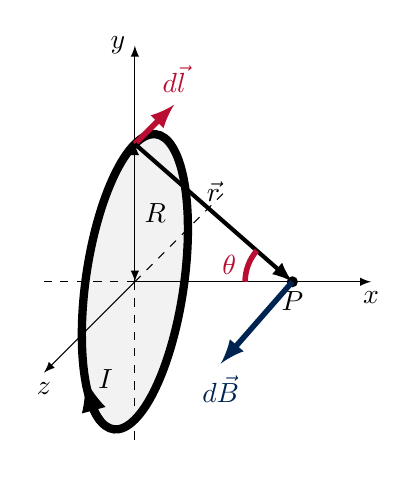
\begin{tikzpicture}[scale=1]

\tikzmath{
\R = 1.75;
\L = 3;
\xp = 2;
\dl = 1.3; 
\dBs = 0.4;
\pa = 0; %phi, position of dl
\dlpx = 0;
\dlpy = cos(\pa)*\R;
\dlpz = sin(\pa)*\R;
%components of dl
\dlx = 0;
\dly = \dl*sin(\pa);
\dlz = -\dl*cos(\pa);
%cone opening angle
\th = atan(\R/\xp);
%r vector for cross-product
\rx = \xp;
\ry = -\dlpy;
\rz = -\dlpz;
\dBx = \dBs*(\dly*\rz-\dlz*\ry);
\dBy = \dBs*(\dlz*\rx-\dlx*\rz);
\dBz = \dBs*(\dlx*\ry-\dly*\rx);
\dBm = sqrt(\dBx*\dBx+\dBy*\dBy+\dBz*\dBz);
\dBr = \dBm*cos(\th);
\dBrx = \xp-\dBm*sin(\th);
}

\coordinate (P) at (\xp,0,0);
\coordinate (PL) at (\dlpx,\dlpy,\dlpz);

%axes:
\draw[-latex] (0,0,0) -- (\L,0,0) node[below] {$x$};
\draw[-latex] (0,0,0) -- (0,\L,0) node[left] {$y$};
\draw[-latex] (0,0,0) -- (0,0,\L) node[below] {$z$};
\draw[dashed] (0,0,0) -- (0,0,-\L);
\draw[dashed] (0,0,0) -- (0,-0.7*\L,0);
\draw[dashed] (0,0,0) -- (-0.4*\L,0,0);
%P
\node[below] at (P) {$P$};
\fill (P) circle(2pt);
%wire:
\begin{scope}[canvas is yz plane at x=0]
\draw[line width=3] (0,0) circle(\R);
\fill[opacity=0.05] (0,0) circle(\R);
\draw[line width=3,-latex] (140:\R) arc (140:110:\R) node[right] {$I$};
\end{scope}

\draw[latex-latex, dotted] (0,0,0) -- (0,\R,0) node[midway,right]{$R$};


%construction
\begin{scope}[canvas is yz plane at x=0]
\draw[-latex,color=qred, line width = 2pt] (\dlpy,\dlpz) -- +(\dly,\dlz) node[above] {$d\vec l$};
\end{scope}

\draw[-latex, line width=1.5pt] (PL) -- (P) node[midway,above] {$\vec r$};

\draw[-latex,color=qblue, line width = 2pt] (P) -- +(\dBx,\dBy,\dBz) node[below] {$d\vec B$};

%angle theta
\draw[color=qred,line width=2pt] (0.7*\xp,0) arc(180:180-\th:0.3*\xp) node[midway,left] {$\theta$};


\end{tikzpicture}
\captionof*{figure}{\textit{Using the Biot-Savart law to determine the magnetic field at point $P$ due to the ring carrying current, $I$.}}
}

%%%%%%%%%%%%%%%%%%%%%%%%%%%%%%  phi=270
\twocolframesf{Magnetic field from a ring of current}
{
\begin{enumerate}
\item Make a good diagram.
\item Choose $d\vec l$.
\item Determine $d \vec l\times \vec r$ : $\rightarrow$ magnitude  $=dl r$.
\item Determine $d\vec B$ : $\rightarrow$ magnitude $=\frac{\mu_0Idl}{4\pi r^2}$.
\item Think about symmetry:
\end{enumerate}
}
{
\centering
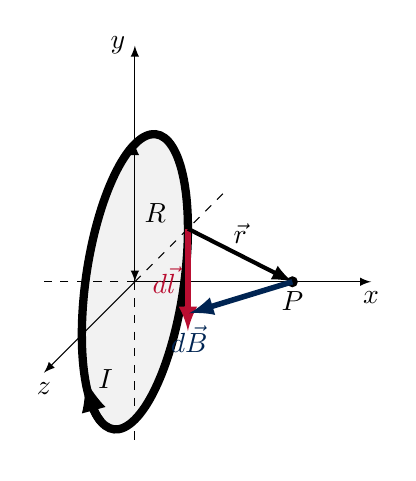
\begin{tikzpicture}[scale=1]

\tikzmath{
\R = 1.75;
\L = 3;
\xp = 2;
\dl = 1.3; 
\dBs = 0.4;
\pa = 270; %phi, position of dl
\dlpx = 0;
\dlpy = cos(\pa)*\R;
\dlpz = sin(\pa)*\R;
%components of dl
\dlx = 0;
\dly = \dl*sin(\pa);
\dlz = -\dl*cos(\pa);
%cone opening angle
\th = atan(\R/\xp);
%r vector for cross-product
\rx = \xp;
\ry = -\dlpy;
\rz = -\dlpz;
\dBx = \dBs*(\dly*\rz-\dlz*\ry);
\dBy = \dBs*(\dlz*\rx-\dlx*\rz);
\dBz = \dBs*(\dlx*\ry-\dly*\rx);
\dBm = sqrt(\dBx*\dBx+\dBy*\dBy+\dBz*\dBz);
\dBr = \dBm*cos(\th);
\dBrx = \xp-\dBm*sin(\th);
}

\coordinate (P) at (\xp,0,0);
\coordinate (PL) at (\dlpx,\dlpy,\dlpz);

%axes:
\draw[-latex] (0,0,0) -- (\L,0,0) node[below] {$x$};
\draw[-latex] (0,0,0) -- (0,\L,0) node[left] {$y$};
\draw[-latex] (0,0,0) -- (0,0,\L) node[below] {$z$};
\draw[dashed] (0,0,0) -- (0,0,-\L);
\draw[dashed] (0,0,0) -- (0,-0.7*\L,0);
\draw[dashed] (0,0,0) -- (-0.4*\L,0,0);
%P
\node[below] at (P) {$P$};
\fill (P) circle(2pt);
%wire:
\begin{scope}[canvas is yz plane at x=0]
\draw[line width=3] (0,0) circle(\R);
\fill[opacity=0.05] (0,0) circle(\R);
\draw[line width=3,-latex] (140:\R) arc (140:110:\R) node[right] {$I$};
\end{scope}

\draw[latex-latex, dotted] (0,0,0) -- (0,\R,0) node[midway,right]{$R$};

%construction
\begin{scope}[canvas is yz plane at x=0]
\draw[-latex,color=qred, line width = 2pt] (\dlpy,\dlpz) -- +(\dly,\dlz) node[midway,left] {$d\vec l$};
\end{scope}

\draw[-latex, line width=1.5pt] (PL) -- (P) node[midway,above] {$\vec r$};

\draw[-latex,color=qblue, line width = 2pt] (P) -- +(\dBx,\dBy,\dBz) node[below] {$d\vec B$};

\end{tikzpicture}
\captionof*{figure}{\textit{Using the Biot-Savart law to determine the magnetic field at point $P$ due to the ring carrying current, $I$.}}

}

%%%%%%%%%%%%%%%%%%%%%%%%%%%%%% phi  180
\twocolframesf{Magnetic field from a ring of current}
{
\begin{enumerate}
\item Make a good diagram.
\item Choose $d\vec l$.
\item Determine $d \vec l\times \vec r$ : $\rightarrow$ magnitude  $=dl r$.
\item Determine $d\vec B$ : $\rightarrow$ magnitude $=\frac{\mu_0Idl}{4\pi r^2}$.
\item Think about symmetry:
\end{enumerate}
}
{
\centering
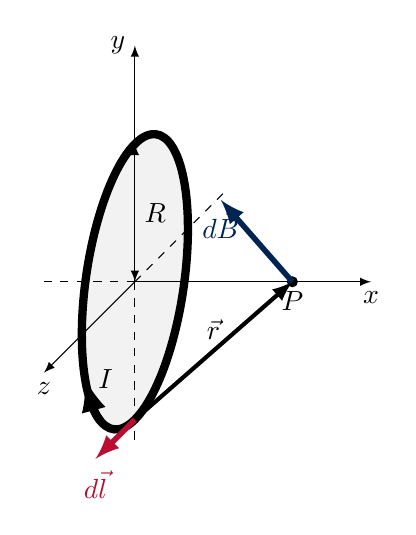
\begin{tikzpicture}[scale=1]

\tikzmath{
\R = 1.75;
\L = 3;
\xp = 2;
\dl = 1.3; 
\dBs = 0.4;
\pa = 180; %phi, position of dl
\dlpx = 0;
\dlpy = cos(\pa)*\R;
\dlpz = sin(\pa)*\R;
%components of dl
\dlx = 0;
\dly = \dl*sin(\pa);
\dlz = -\dl*cos(\pa);
%cone opening angle
\th = atan(\R/\xp);
%r vector for cross-product
\rx = \xp;
\ry = -\dlpy;
\rz = -\dlpz;
\dBx = \dBs*(\dly*\rz-\dlz*\ry);
\dBy = \dBs*(\dlz*\rx-\dlx*\rz);
\dBz = \dBs*(\dlx*\ry-\dly*\rx);
\dBm = sqrt(\dBx*\dBx+\dBy*\dBy+\dBz*\dBz);
\dBr = \dBm*cos(\th);
\dBrx = \xp-\dBm*sin(\th);
}

\coordinate (P) at (\xp,0,0);
\coordinate (PL) at (\dlpx,\dlpy,\dlpz);

%axes:
\draw[-latex] (0,0,0) -- (\L,0,0) node[below] {$x$};
\draw[-latex] (0,0,0) -- (0,\L,0) node[left] {$y$};
\draw[-latex] (0,0,0) -- (0,0,\L) node[below] {$z$};
\draw[dashed] (0,0,0) -- (0,0,-\L);
\draw[dashed] (0,0,0) -- (0,-0.7*\L,0);
\draw[dashed] (0,0,0) -- (-0.4*\L,0,0);
%P
\node[below] at (P) {$P$};
\fill (P) circle(2pt);
%wire:
\begin{scope}[canvas is yz plane at x=0]
\draw[line width=3] (0,0) circle(\R);
\fill[opacity=0.05] (0,0) circle(\R);
\draw[line width=3,-latex] (140:\R) arc (140:110:\R) node[right] {$I$};
\end{scope}

\draw[latex-latex, dotted] (0,0,0) -- (0,\R,0) node[midway,right]{$R$};

%construction
\begin{scope}[canvas is yz plane at x=0]
\draw[-latex,color=qred, line width = 2pt] (\dlpy,\dlpz) -- +(\dly,\dlz) node[below] {$d\vec l$};
\end{scope}

\draw[-latex, line width=1.5pt] (PL) -- (P) node[midway,above] {$\vec r$};

\draw[-latex,color=qblue, line width = 2pt] (P) -- +(\dBx,\dBy,\dBz) node[below] {$d\vec B$};

\end{tikzpicture}
\captionof*{figure}{\textit{Using the Biot-Savart law to determine the magnetic field at point $P$ due to the ring carrying current, $I$.}}
}

%%%%%%%%%%%%%%%%%%%%%%%%%%%%%% phi = 90
\twocolframesf{Magnetic field from a ring of current}
{
\begin{enumerate}
\item Make a good diagram.
\item Choose $d\vec l$.
\item Determine $d \vec l\times \vec r$ : $\rightarrow$ magnitude  $=dl r$.
\item Determine $d\vec B$ : $\rightarrow$ magnitude $=\frac{\mu_0Idl}{4\pi r^2}$.
\item Think about symmetry:
\end{enumerate}
}
{
\centering
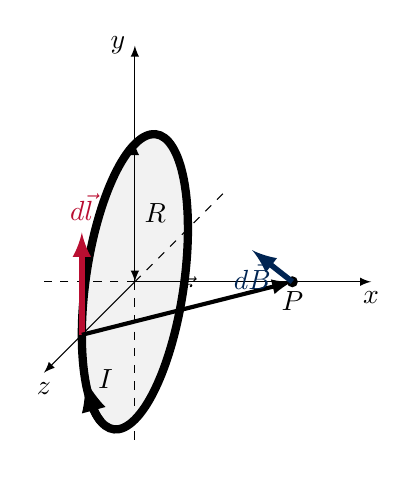
\begin{tikzpicture}[scale=1]

\tikzmath{
\R = 1.75;
\L = 3;
\xp = 2;
\dl = 1.3; 
\dBs = 0.4;
\pa = 90; %phi, position of dl
\dlpx = 0;
\dlpy = cos(\pa)*\R;
\dlpz = sin(\pa)*\R;
%components of dl
\dlx = 0;
\dly = \dl*sin(\pa);
\dlz = -\dl*cos(\pa);
%cone opening angle
\th = atan(\R/\xp);
%r vector for cross-product
\rx = \xp;
\ry = -\dlpy;
\rz = -\dlpz;
\dBx = \dBs*(\dly*\rz-\dlz*\ry);
\dBy = \dBs*(\dlz*\rx-\dlx*\rz);
\dBz = \dBs*(\dlx*\ry-\dly*\rx);
\dBm = sqrt(\dBx*\dBx+\dBy*\dBy+\dBz*\dBz);
\dBr = \dBm*cos(\th);
\dBrx = \xp-\dBm*sin(\th);
}

\coordinate (P) at (\xp,0,0);
\coordinate (PL) at (\dlpx,\dlpy,\dlpz);

%axes:
\draw[-latex] (0,0,0) -- (\L,0,0) node[below] {$x$};
\draw[-latex] (0,0,0) -- (0,\L,0) node[left] {$y$};
\draw[-latex] (0,0,0) -- (0,0,\L) node[below] {$z$};
\draw[dashed] (0,0,0) -- (0,0,-\L);
\draw[dashed] (0,0,0) -- (0,-0.7*\L,0);
\draw[dashed] (0,0,0) -- (-0.4*\L,0,0);
%P
\node[below] at (P) {$P$};
\fill (P) circle(2pt);
%wire:
\begin{scope}[canvas is yz plane at x=0]
\draw[line width=3] (0,0) circle(\R);
\fill[opacity=0.05] (0,0) circle(\R);
\draw[line width=3,-latex] (140:\R) arc (140:110:\R) node[right] {$I$};
\end{scope}

\draw[latex-latex, dotted] (0,0,0) -- (0,\R,0) node[midway,right]{$R$};

%construction
\begin{scope}[canvas is yz plane at x=0]
\draw[-latex,color=qred, line width = 2pt] (\dlpy,\dlpz) -- +(\dly,\dlz) node[above] {$d\vec l$};
\end{scope}
\draw[-latex, line width=1.5pt] (PL) -- (P) node[midway,above] {$\vec r$};
\draw[-latex,color=qblue, line width = 2pt] (P) -- +(\dBx,\dBy,\dBz) node[below] {$d\vec B$};

\end{tikzpicture}
\captionof*{figure}{\textit{Using the Biot-Savart law to determine the magnetic field at point $P$ due to the ring carrying current, $I$.}}
}

%%%%%%%%%%%%%%%%%%%%%%%%%%%%%% with circle
\twocolframesf{Magnetic field from a ring of current}
{
\begin{enumerate}
\item Make a good diagram.
\item Choose $d\vec l$.
\item Determine $d \vec l\times \vec r$ : $\rightarrow$ magnitude  $=dl r$.
\item Determine $d\vec B$ : $\rightarrow$ magnitude $=\frac{\mu_0Idl}{4\pi r^2}$.
\item Think about symmetry:
\end{enumerate}
\emph{The tip of the magnetic field vector traces out a circle. Only the component along $-x$ will survive the integral. }
}
{
\centering
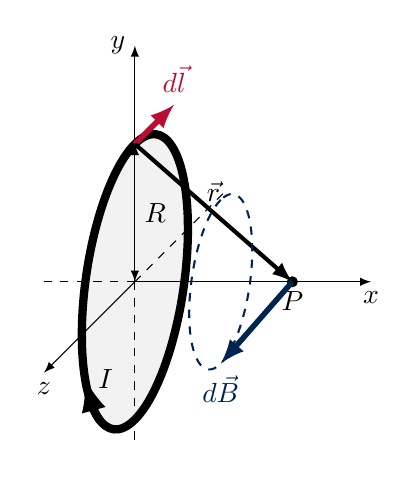
\begin{tikzpicture}[scale=1]

\tikzmath{
\R = 1.75;
\L = 3;
\xp = 2;
\dl = 1.3; 
\dBs = 0.4;
\pa = 0; %phi, position of dl
\dlpx = 0;
\dlpy = cos(\pa)*\R;
\dlpz = sin(\pa)*\R;
%components of dl
\dlx = 0;
\dly = \dl*sin(\pa);
\dlz = -\dl*cos(\pa);
%cone opening angle
\th = atan(\R/\xp);
%r vector for cross-product
\rx = \xp;
\ry = -\dlpy;
\rz = -\dlpz;
\dBx = \dBs*(\dly*\rz-\dlz*\ry);
\dBy = \dBs*(\dlz*\rx-\dlx*\rz);
\dBz = \dBs*(\dlx*\ry-\dly*\rx);
\dBm = sqrt(\dBx*\dBx+\dBy*\dBy+\dBz*\dBz);
\dBr = \dBm*cos(\th);
\dBrx = \xp-\dBm*sin(\th);
}

\coordinate (P) at (\xp,0,0);
\coordinate (PL) at (\dlpx,\dlpy,\dlpz);

%axes:
\draw[-latex] (0,0,0) -- (\L,0,0) node[below] {$x$};
\draw[-latex] (0,0,0) -- (0,\L,0) node[left] {$y$};
\draw[-latex] (0,0,0) -- (0,0,\L) node[below] {$z$};
\draw[dashed] (0,0,0) -- (0,0,-\L);
\draw[dashed] (0,0,0) -- (0,-0.7*\L,0);
\draw[dashed] (0,0,0) -- (-0.4*\L,0,0);
%P
\node[below] at (P) {$P$};
\fill (P) circle(2pt);
%wire:
\begin{scope}[canvas is yz plane at x=0]
\draw[line width=3] (0,0) circle(\R);
\fill[opacity=0.05] (0,0) circle(\R);
\draw[line width=3,-latex] (140:\R) arc (140:110:\R) node[right] {$I$};
\end{scope}

\draw[latex-latex, dotted] (0,0,0) -- (0,\R,0) node[midway,right]{$R$};

%construction
\begin{scope}[canvas is yz plane at x=0]
\draw[-latex,color=qred, line width = 2pt] (\dlpy,\dlpz) -- +(\dly,\dlz) node[above] {$d\vec l$};
\end{scope}

\draw[-latex, line width=1.5pt] (PL) -- (P) node[midway,above] {$\vec r$};

\draw[-latex,color=qblue, line width = 2pt] (P) -- +(\dBx,\dBy,\dBz) node[below] {$d\vec B$};
%circle for tip of B
\begin{scope}[canvas is yz plane at x=\dBrx]
\draw[color=qblue, line width = 0.75pt, dashed] (0,0) circle(\dBr);
\end{scope}

\end{tikzpicture}
\captionof*{figure}{\textit{Using the Biot-Savart law to determine the magnetic field at point $P$ due to the ring carrying current, $I$.}}

}

%%%%%%%%%%%%%%%%%%%%%%%%%%%%%%
%%%%%%%%%%%%%%%%%%%%%%%%%%%%%%%%%%%
%%%%%% animation
%%%%%%%%%%%%%%%%%%%%%%%%%%%%%%%%%%%
\begin{frame}
\centering
\pgfmathtruncatemacro\N{40}
\begin{animateinline}[controls,loop]{5} % 5 fps, same as 0.2 s transduration

\multiframe{\N}{i=0+1}{

\begin{tikzpicture}[scale=1]

\tikzmath{
\R = 1.75;
\L = 3;
\xp = 2;
\dl = 1.3; 
\dBs = 0.4;
\pa = -\i*360/\N; %phi, position of dl
\dlpx = 0;
\dlpy = cos(\pa)*\R;
\dlpz = sin(\pa)*\R;
%components of dl
\dlx = 0;
\dly = \dl*sin(\pa);
\dlz = -\dl*cos(\pa);
%cone opening angle
\th = atan(\R/\xp);
%r vector for cross-product
\rx = \xp;
\ry = -\dlpy;
\rz = -\dlpz;
\dBx = \dBs*(\dly*\rz-\dlz*\ry);
\dBy = \dBs*(\dlz*\rx-\dlx*\rz);
\dBz = \dBs*(\dlx*\ry-\dly*\rx);
\dBm = sqrt(\dBx*\dBx+\dBy*\dBy+\dBz*\dBz);
\dBr = \dBm*cos(\th);
\dBrx = \xp-\dBm*sin(\th);
}

\coordinate (P) at (\xp,0,0);
\coordinate (PL) at (\dlpx,\dlpy,\dlpz);

%axes:
\draw[-latex] (0,0,0) -- (\L,0,0) node[below] {$x$};
\draw[-latex] (0,0,0) -- (0,\L,0) node[left] {$y$};
\draw[-latex] (0,0,0) -- (0,0,\L) node[below] {$z$};
\draw[dashed] (0,0,0) -- (0,0,-\L);
\draw[dashed] (0,0,0) -- (0,-0.7*\L,0);
\draw[dashed] (0,0,0) -- (-0.4*\L,0,0);
%P
\node[below] at (P) {$P$};
\fill (P) circle(2pt);
%wire:
\begin{scope}[canvas is yz plane at x=0]
\draw[line width=3] (0,0) circle(\R);
\fill[opacity=0.05] (0,0) circle(\R);
\draw[line width=3,-latex] (140:\R) arc (140:110:\R) node[right] {$I$};
\end{scope}

%construction
\begin{scope}[canvas is yz plane at x=0]
\draw[-latex,color=qred, line width = 2pt] (\dlpy,\dlpz) -- +(\dly,\dlz) node[above] {$d\vec l$};
\end{scope}

\draw[latex-latex, dotted] (0,0,0) -- (0,\R,0) node[midway,right]{$R$};

\draw[-latex, line width=1.5pt] (PL) -- (P) node[midway,above] {$\vec r$};

\draw[-latex,color=qblue, line width = 2pt] (P) -- +(\dBx,\dBy,\dBz) node[below] {$d\vec B$};
%circle for tip of B
\begin{scope}[canvas is yz plane at x=\dBrx]
\draw[color=qblue, line width = 0.75pt, dashed] (0,0) circle(\dBr);
\end{scope}

\end{tikzpicture}

}
\end{animateinline}
\end{frame}


%%%%%%%%%%%%%%%%%%%%%%%%%%%%%% with circle

\twocolframesf{Magnetic field from a ring of current}
{
\begin{enumerate}
\item Make a good diagram.
\item Choose $d\vec l$.
\item Determine $d \vec l\times \vec r$ : $\rightarrow$ magnitude  $=dl r$.
\item Determine $d\vec B$ : $\rightarrow$ magnitude $=\frac{\mu_0Idl}{4\pi r^2}$.
\item Think about symmetry:
\end{enumerate}
Only the $x$ component of the $d\vec B$ don't cancel out:
\only<1>{
\begin{align*}
dB_x=dB\cos\dots
\end{align*}
}
\only<2>{
\begin{align*}
dB_x=dB\cos\left(\frac{\pi}{2}-\theta\right)=dB\sin\theta
\end{align*}
}
}
{
\centering
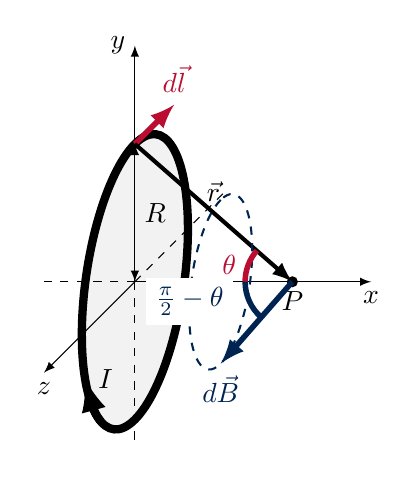
\begin{tikzpicture}[scale=1]

\tikzmath{
\R = 1.75;
\L = 3;
\xp = 2;
\dl = 1.3; 
\dBs = 0.4;
\pa = 0; %phi, position of dl
\dlpx = 0;
\dlpy = cos(\pa)*\R;
\dlpz = sin(\pa)*\R;
%components of dl
\dlx = 0;
\dly = \dl*sin(\pa);
\dlz = -\dl*cos(\pa);
%cone opening angle
\th = atan(\R/\xp);
%r vector for cross-product
\rx = \xp;
\ry = -\dlpy;
\rz = -\dlpz;
\dBx = \dBs*(\dly*\rz-\dlz*\ry);
\dBy = \dBs*(\dlz*\rx-\dlx*\rz);
\dBz = \dBs*(\dlx*\ry-\dly*\rx);
\dBm = sqrt(\dBx*\dBx+\dBy*\dBy+\dBz*\dBz);
\dBr = \dBm*cos(\th);
\dBrx = \xp-\dBm*sin(\th);
}

\coordinate (P) at (\xp,0,0);
\coordinate (PL) at (\dlpx,\dlpy,\dlpz);

%axes:
\draw[-latex] (0,0,0) -- (\L,0,0) node[below] {$x$};
\draw[-latex] (0,0,0) -- (0,\L,0) node[left] {$y$};
\draw[-latex] (0,0,0) -- (0,0,\L) node[below] {$z$};
\draw[dashed] (0,0,0) -- (0,0,-\L);
\draw[dashed] (0,0,0) -- (0,-0.7*\L,0);
\draw[dashed] (0,0,0) -- (-0.4*\L,0,0);
%P
\node[below] at (P) {$P$};
\fill (P) circle(2pt);
%wire:
\begin{scope}[canvas is yz plane at x=0]
\draw[line width=3] (0,0) circle(\R);
\fill[opacity=0.05] (0,0) circle(\R);
\draw[line width=3,-latex] (140:\R) arc (140:110:\R) node[right] {$I$};
\end{scope}

%construction
\begin{scope}[canvas is yz plane at x=0]
\draw[-latex,color=qred, line width = 2pt] (\dlpy,\dlpz) -- +(\dly,\dlz) node[above] {$d\vec l$};
\end{scope}
\draw[latex-latex, dotted] (0,0,0) -- (0,\R,0) node[midway,right]{$R$};

\draw[-latex, line width=1.5pt] (PL) -- (P) node[midway,above] {$\vec r$};

\draw[-latex,color=qblue, line width = 2pt] (P) -- +(\dBx,\dBy,\dBz) node[below] {$d\vec B$};
%circle for tip of B
\begin{scope}[canvas is yz plane at x=\dBrx]
\draw[color=qblue, line width = 0.75pt, dashed] (0,0) circle(\dBr);
\end{scope}

%angle theta
\draw[color=qred,line width=2pt] (0.7*\xp,0) arc(180:180-\th:0.3*\xp) node[midway,left] {$\theta$};
%angle  90 -theta
\only<2>{
\draw[color=qblue,line width=2pt] (0.7*\xp,0) arc(180:180+90-\th:0.3*\xp) node[fill=white,midway,left=5pt] {$\frac{\pi}{2}-\theta$};
}

\end{tikzpicture}
\captionof*{figure}{\textit{Using the Biot-Savart law to determine the magnetic field at point $P$ due to the ring carrying current, $I$.}}

}


%%%%%%%%%%%%%%%%%%%%%%%%%%%%%% Finally

\twocolframesf{Magnetic field from a ring of current}
{
\begin{enumerate}
\item Make a good diagram.
\item Choose $d\vec l$.
\item Determine $d \vec l\times \vec r$ : $\rightarrow$ magnitude  $=dl r$.
\item Determine $d\vec B$ : $\rightarrow$ magnitude $=\frac{\mu_0Idl}{4\pi r^2}$.
\item Think about symmetry: $dB_x=dB\sin\theta$
\end{enumerate}
All together:
\begin{align*}
B_x = \int dB_x = \int dB\sin\theta =  \frac{\mu_0I}{4\pi}\int \frac{1}{r^2}\sin\theta dl
\end{align*}
\only<3>{
\begin{align*}
= \frac{\mu_0I}{4\pi r^2}\sin\theta  \int_0^{2\pi R} dl = \frac{\mu_0I}{4\pi r^2}\sin\theta (2\pi R)
\end{align*}
}
}
{
\centering
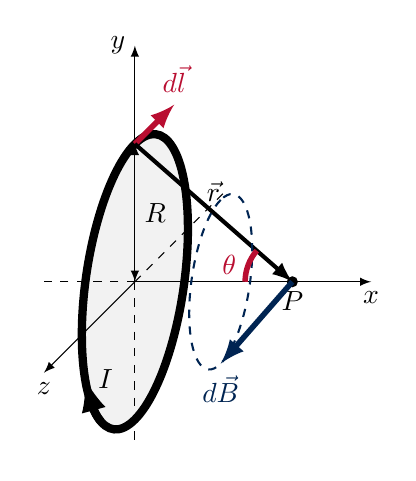
\begin{tikzpicture}[scale=1]

\tikzmath{
\R = 1.75;
\L = 3;
\xp = 2;
\dl = 1.3; 
\dBs = 0.4;
\pa = 0; %phi, position of dl
\dlpx = 0;
\dlpy = cos(\pa)*\R;
\dlpz = sin(\pa)*\R;
%components of dl
\dlx = 0;
\dly = \dl*sin(\pa);
\dlz = -\dl*cos(\pa);
%cone opening angle
\th = atan(\R/\xp);
%r vector for cross-product
\rx = \xp;
\ry = -\dlpy;
\rz = -\dlpz;
\dBx = \dBs*(\dly*\rz-\dlz*\ry);
\dBy = \dBs*(\dlz*\rx-\dlx*\rz);
\dBz = \dBs*(\dlx*\ry-\dly*\rx);
\dBm = sqrt(\dBx*\dBx+\dBy*\dBy+\dBz*\dBz);
\dBr = \dBm*cos(\th);
\dBrx = \xp-\dBm*sin(\th);
}

\coordinate (P) at (\xp,0,0);
\coordinate (PL) at (\dlpx,\dlpy,\dlpz);

%axes:
\draw[-latex] (0,0,0) -- (\L,0,0) node[below] {$x$};
\draw[-latex] (0,0,0) -- (0,\L,0) node[left] {$y$};
\draw[-latex] (0,0,0) -- (0,0,\L) node[below] {$z$};
\draw[dashed] (0,0,0) -- (0,0,-\L);
\draw[dashed] (0,0,0) -- (0,-0.7*\L,0);
\draw[dashed] (0,0,0) -- (-0.4*\L,0,0);
%P
\node[below] at (P) {$P$};
\fill (P) circle(2pt);
%wire:
\begin{scope}[canvas is yz plane at x=0]
\draw[line width=3] (0,0) circle(\R);
\fill[opacity=0.05] (0,0) circle(\R);
\draw[line width=3,-latex] (140:\R) arc (140:110:\R) node[right] {$I$};
\end{scope}

%construction
\begin{scope}[canvas is yz plane at x=0]
\draw[-latex,color=qred, line width = 2pt] (\dlpy,\dlpz) -- +(\dly,\dlz) node[above] {$d\vec l$};
\end{scope}

\draw[latex-latex, dotted] (0,0,0) -- (0,\R,0) node[midway,right]{$R$};

\draw[-latex, line width=1.5pt] (PL) -- (P) node[midway,above] {$\vec r$};

\draw[-latex,color=qblue, line width = 2pt] (P) -- +(\dBx,\dBy,\dBz) node[below] {$d\vec B$};
%circle for tip of B
\begin{scope}[canvas is yz plane at x=\dBrx]
\draw[color=qblue, line width = 0.75pt, dashed] (0,0) circle(\dBr);
\end{scope}

%angle theta
\draw[color=qred,line width=2pt] (0.7*\xp,0) arc(180:180-\th:0.3*\xp) node[midway,left] {$\theta$};
%angle  90 -theta

\end{tikzpicture}
\captionof*{figure}{\textit{Using the Biot-Savart law to determine the magnetic field at point $P$ due to the ring carrying current, $I$.}}

}


%%%%%%%%%%%%%%%%%%%%%%%%%%%%%% Finally

\twocolframesf{Magnetic field from a ring of current}
{
And, finally, with $P$ located a distance $x$ from the origin:
\begin{align*}
B_x &= -\frac{\mu_0I}{4\pi r^2}\sin\theta (2\pi R)\\
r &= \sqrt{R^2+x^2}\\
\sin\theta&=\frac{R}{r}=\frac{R}{\sqrt{R^2+x^2}}
\end{align*}
\begin{align*}
\boxed{\vec B = -\frac{\mu_0I}{2}\frac{R^2}{(R^2+x^2)^{\frac{3}{2}}} \hat x}
\end{align*}
}
{
\centering
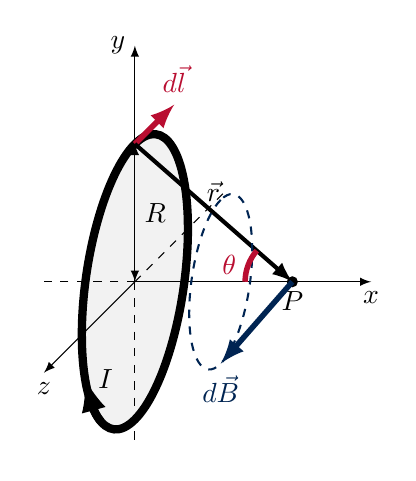
\begin{tikzpicture}[scale=1]

\tikzmath{
\R = 1.75;
\L = 3;
\xp = 2;
\dl = 1.3; 
\dBs = 0.4;
\pa = 0; %phi, position of dl
\dlpx = 0;
\dlpy = cos(\pa)*\R;
\dlpz = sin(\pa)*\R;
%components of dl
\dlx = 0;
\dly = \dl*sin(\pa);
\dlz = -\dl*cos(\pa);
%cone opening angle
\th = atan(\R/\xp);
%r vector for cross-product
\rx = \xp;
\ry = -\dlpy;
\rz = -\dlpz;
\dBx = \dBs*(\dly*\rz-\dlz*\ry);
\dBy = \dBs*(\dlz*\rx-\dlx*\rz);
\dBz = \dBs*(\dlx*\ry-\dly*\rx);
\dBm = sqrt(\dBx*\dBx+\dBy*\dBy+\dBz*\dBz);
\dBr = \dBm*cos(\th);
\dBrx = \xp-\dBm*sin(\th);
}

\coordinate (P) at (\xp,0,0);
\coordinate (PL) at (\dlpx,\dlpy,\dlpz);

%axes:
\draw[-latex] (0,0,0) -- (\L,0,0) node[below] {$x$};
\draw[-latex] (0,0,0) -- (0,\L,0) node[left] {$y$};
\draw[-latex] (0,0,0) -- (0,0,\L) node[below] {$z$};
\draw[dashed] (0,0,0) -- (0,0,-\L);
\draw[dashed] (0,0,0) -- (0,-0.7*\L,0);
\draw[dashed] (0,0,0) -- (-0.4*\L,0,0);
%P
\node[below] at (P) {$P$};
\fill (P) circle(2pt);
%wire:
\begin{scope}[canvas is yz plane at x=0]
\draw[line width=3] (0,0) circle(\R);
\fill[opacity=0.05] (0,0) circle(\R);
\draw[line width=3,-latex] (140:\R) arc (140:110:\R) node[right] {$I$};
\end{scope}

%construction
\begin{scope}[canvas is yz plane at x=0]
\draw[-latex,color=qred, line width = 2pt] (\dlpy,\dlpz) -- +(\dly,\dlz) node[above] {$d\vec l$};
\end{scope}

\draw[latex-latex, dotted] (0,0,0) -- (0,\R,0) node[midway,right]{$R$};

\draw[-latex, line width=1.5pt] (PL) -- (P) node[midway,above] {$\vec r$};

\draw[-latex,color=qblue, line width = 2pt] (P) -- +(\dBx,\dBy,\dBz) node[below] {$d\vec B$};
%circle for tip of B
\begin{scope}[canvas is yz plane at x=\dBrx]
\draw[color=qblue, line width = 0.75pt, dashed] (0,0) circle(\dBr);
\end{scope}

%angle theta
\draw[color=qred,line width=2pt] (0.7*\xp,0) arc(180:180-\th:0.3*\xp) node[midway,left] {$\theta$};
%angle  90 -theta

\end{tikzpicture}
\captionof*{figure}{\textit{Using the Biot-Savart law to determine the magnetic field at point $P$ due to the ring carrying current, $I$.}}

}
%%%%%%%%%%%%%%%%%%%%%%%%%%%%%%
%%% End of ring
%%%%%%%%%%%%%%%%%%%%%%%%%%%%%%


%%%%%%%%%%%%%%%%%%%%%%%%%%%%%%%%
\section{Ampère's Law}
\label{sec:ampereslaw}
\title{Ampère's Law}


%%%%%%%%%%%%%%%%%%%%%%%%%
\begin{frame}
\titlepage
\thispagestyle{empty}
\end{frame}

%%%%%%%%%%%%%%%%%%%%%%%%%%


%%%%%%%%%%%%%%%%%%%%%%%%%%%%%%
\subsection{Formula}
\label{subsec:alawformula}
\begin{frame}{Ampère's Law}
Ampère's Law:
\begin{align*}
\oint \vec B \cdot d\vec l = \mu_0I^{enc}
\end{align*}
Similar to Gauss' Law:
\begin{align*}
\oint \vec E \cdot d\vec A = \frac{Q^{enc}}{\epsilon_0}
\end{align*}
Except:
\begin{itemize}
\item Integral is over a path ($d\vec l$), not a surface. 
\item Related to current enclosed by a \emph{closed loop} instead of charge enclosed by a closed surface.
\end{itemize}
\end{frame}



%%%%%%%%%%%%%%%%%%%%%%%%%%%%%%
\subsection{The path integral}
\label{subsec:thepathintegral}
\begin{frame}{The path integral, $\oint \vec B \cdot d\vec l$}
\begin{itemize}
\item We have seen path integrals in the context of work:
\begin{align*}
W = \int_A^B \vec F \cdot d\vec l
\end{align*}
\item The circle sign just means that it's a closed path, $A=B$. We know that for a conservative force, $\vec F$:
\begin{align*}
 \oint \vec F \cdot d\vec l = 0 \quad \text{(conservative force)}
\end{align*}
\end{itemize}
\end{frame}


%%%%%%%%%%%%%%%%%%%%%%%%%%%%%%



%%%%%%%%%%%%%%%%%%%%%%%%%%%%%%
\subsection{Field near an infinite current-carrying wire}
\label{subsec:fieldnearaninfinitecurrentcarryingwire}
\twocolframesf{Example: Field near an infinite current-carrying wire}
{
\begin{enumerate}
\item Use symmetry to determine the direction of $\vec B$.
\item<2-> Choose a path where the integral $\oint \vec B \cdot d\vec l$ is easy
\only<2>{
\begin{itemize}
\item $\vec B$ and $d\vec l$ make constant angle along path.
\item $\vec B$ doesn't change magnitude along path.
\end{itemize}
$\rightarrow$ choose a circle of radius $r$ centred on the wire!
}
\item<3-> Evalulate the integral:
\begin{align*}
\oint \vec B \cdot d\vec l=\oint Bdl = B\oint dl =B2\pi r
\end{align*}

\item<4-> Determine the enclosed current: $I^{enc}=I$ (it's all enclosed!)
\item<5-> Apply Ampère's Law:
\begin{align*}
\oint \vec B \cdot d\vec l = \mu_0I^{enc}\;\; \rightarrow 
B2\pi r=\mu_0I \;\; \rightarrow B = \frac{\mu_0 I}{2\pi r}
\end{align*}

\end{enumerate}
}
{
\centering
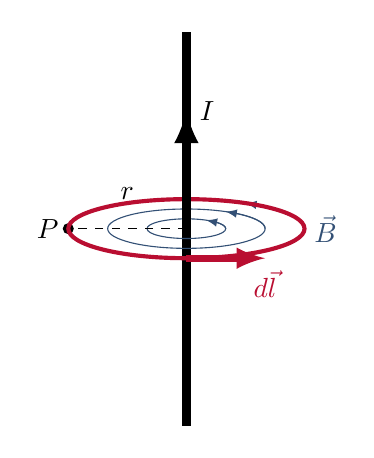
\begin{tikzpicture}[scale=1]
\def\L{5}
\def\D{1}

\draw[line width =3] (0,-\L/2) -- (0,\L/2);

\draw[color=qblue!80] (0,0) circle [x radius=0.5*\D, y radius=0.5*\D/4];
\draw[-latex, color=qblue!80] (0.5*\D,0) arc(0:60:{0.5*\D} and {0.5*\D/4});
\draw[color=qblue!80] (0,0) circle [x radius=\D, y radius=\D/4];
\draw[-latex, color=qblue!80] (1.0*\D,0) arc(0:60:{1.0*\D} and {1.0*\D/4});
\draw[color=qblue!80] (0,0) circle [x radius=1.5*\D, y radius=1.5*\D/4];
\draw[-latex, color=qblue!80] (1.5*\D,0) arc(0:60:{1.5*\D} and {1.5*\D/4});
\node[right, color=qblue!80] at (1.5*\D,0) {$\vec B$};
\draw[dashed] (0,0) -- (-1.5*\D,0) node[midway,above=7pt] {$r$};
\fill (-1.5*\D,0) circle(2pt);
\node[left] at (-1.5*\D,0) {$P$};
\draw[-latex,line width =3] (0,0) -- (0,0.3*\L) node[right]{$I$};


%Ampere loop
\only<2->{
\draw[color=qred, line width = 1.5pt] (0,0) circle [x radius=1.5*\D, y radius=1.5*\D/4];
\draw[-latex,color=qred,line width = 2.5pt](0,-1.5*\D/4) -- +(\D,0) node[below]{$d\vec l$};
\draw[line width =3] (0,0) -- (0,\L/2);
}


\end{tikzpicture}
\captionof*{figure}{\textit{Magnetic field forms concentric circles around the wire.}}
}


%%%%%%%%%%%%%%%%%%%%%%%%%%%%%%
\subsection{Comparing Guass and Ampère's Laws}
\label{subsec:comparinggaussandampereslaws}
\twocolframe{Comparing Gauss and Ampère's Laws}
{
\textbf{Gauss}
\begin{itemize}
\item Need high degree of symmetry
\item Choose a \textbf{surface} that exploits that symmetry:
\begin{itemize}
\item Want field constant in magnitude along surface, and makes a constant angle with surface element, $d\vec A$.
\end{itemize}
\item Calculate \textbf{flux:}
\begin{align*}
\oint \vec E \cdot d\vec A = E\cos\theta\oint dA
\end{align*}
\item Calculate \textbf{charge} enclosed by the closed surface
\end{itemize}
Flux represents field lines coming out of a surface.
}
{
\textbf{Ampère}
\begin{itemize}
\item Need high degree of symmetry
\item Choose a \textbf{loop} that exploits that symmetry:
\begin{itemize}
\item Want field constant in magnitude along loop, and makes a constant angle with path element, $d\vec l$.
\end{itemize}
\item Calculate \textbf{circulation:}
\begin{align*}
\oint \vec B \cdot d\vec l = B\cos\theta\oint dl
\end{align*}
\item Calculate \textbf{current} enclosed by the closed loop.
\end{itemize}
Circulation represents rotation in a field.
}





%%%%%%%%%%%%%%%%%%%%%%%%

\subsection{Circulation of a field}
\label{subsec:circulationofafield}
\begin{frame}{Circulation of a field}
%%%%%%%%%%circulation
\begin{columns}[T]
\column{0.5\textwidth}
\centering
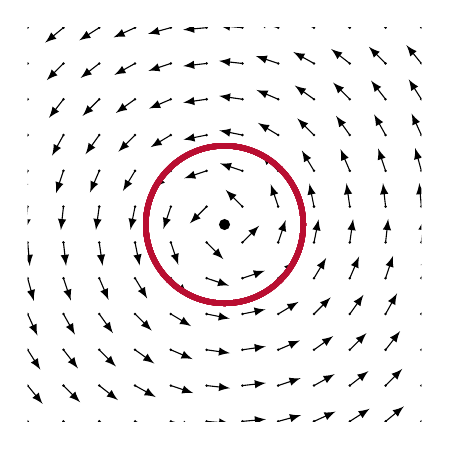
\begin{tikzpicture}[scale=1.0]

\tikzmath{
\L = 5;
\Nl = 11;
\al = 0.3; %arrow length
}

\clip (-\L/2,-\L/2) rectangle (\L/2,\L/2);
\fill (0,0) circle (2pt);

\foreach \i in {0, ..., \Nl}{
  \def\xi{-\L/2+\i*\L/\Nl}
  \foreach \j in {0, ..., \Nl}{
   \def\yj{-\L/2+\j*\L/\Nl}
    
   \def\r{sqrt({\xi}*{\xi}+{\yj}*{\yj})}    
   \def\ux{{-\yj}/{\r}}
   \def\uy{{\xi}/{\r}}
   
   \tikzmath{%unit vector perpendicular to position vector...
    \x = -\L/2+\i*\L/\Nl;
    \y = -\L/2+\j*\L/\Nl;
    \r = sqrt(\x*\x+\y*\y);
    \ux = -\y/\r;
    \uy = \x/\r;
   }
    
   \fill (\x,\y) circle(0.5pt);   
   \draw[-latex] (\xi,\yj) -- ($(\xi,\yj)+({\al*\ux},{\al*\uy})$); 

  }
  \draw[color=qred, line width =2pt] (0,0) circle (\L/5);
}

\end{tikzpicture}
\captionof*{figure}{\textit{Field with circulation and no flux.}}
%%%%%%%%%%%%no circulation
\column{0.5\textwidth}
\centering
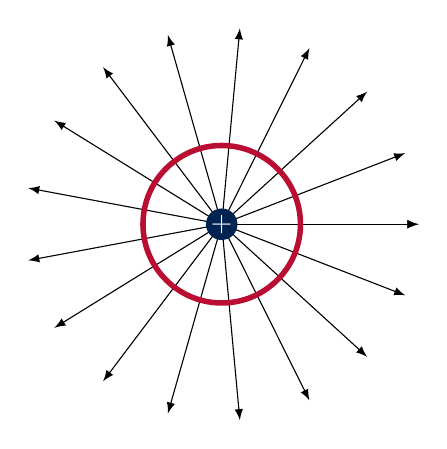
\begin{tikzpicture}[scale=1]

\tikzmath{
\L = 2.5;
\R = 0.2;%charge radius
\Nt = 17;
}

\foreach \i in {0,...,\Nt}{
\def\th{\i*360/\Nt}
\draw [-latex] (0,0) -- (\th:\L);
}
\fill[qblue] (0,0) circle (\R);
\node[white] at (0,0) {$+$};
\draw[color=qred, line width =2pt] (0,0) circle (2*\L/5);

\end{tikzpicture}
\captionof*{figure}{\textit{Field with flux and no circulation.}}
\end{columns}
\begin{itemize}
\item Circulation picks out the component of the field tangent to the path (scalar product picks out parallel components of vectors)
\end{itemize}

\end{frame}


%%%%%%%%%%%%%%%%%%%%%%%%%%%%%%

%%%%%%%%%%%%%%%%%%%%%%%%%%%%%%


%%%%%%%%%%%%%%%%%%%%%%%%%%%%%%%%
\section{Solenoids}
\label{sec:solenoids}
\title{Solenoids}


%%%%%%%%%%%%%%%%%%%%%%%%%
\begin{frame}
\titlepage
\thispagestyle{empty}
\end{frame}

%%%%%%%%%%%%%%%%%%%%%%%%%%


%%%%%%%%%%%%%%%%%%%%%%%%%%%%%%
\subsection{How to build a solenoid}
\label{subsec:howtobuildasolenoid}
\twocolframesf{Solenoids}
{
\begin{itemize}
\item Field from one loop of current, a distance $x$ from centre along axis of symmetry:
\begin{align*}
\vec B = -\frac{\mu_0I}{2}\frac{R^2}{(R^2 + x^2)^\frac{3}{2}} \hat x
\end{align*}

\item<2> By adding more coils, we can get a stronger magnetic field
\end{itemize}
}
{
\centering
\begin{tikzpicture}[scale=1]

\tikzmath{
\R = 2.5;%charge radius
\f = 0.25;
\L = 1;
\Nt = 5;
}

\draw[-latex] (0,0) -- (0,1.25*\R) node[left] {$y$};
\draw[-latex] (0,0) -- (1.25*\R,0) node[below] {$x$};

\only<1>{
%\draw[line width=2] (0,0) circle[x radius={\f*\R}, y radius=\R];

\draw[line width=2] (0,-\R) arc(270:90:{\R*\f} and {\R});
\draw[line width=1.5, dotted] (0,\R) arc(90:-90:{\R*\f} and {\R});

\draw[-latex, line width=2] (-\f*\R,0) -- +(0,0.5) node [right] {$I$};
\draw[-latex, line width =2, color = qblue] (1.1*\R,0) -- + (-0.25*\R,0) node[below] {$\vec B$};
}

\only<2>{
\foreach \i in {0,...,\Nt}{
 \tikzmath{
 \h = -\L/2+\i*\L/\Nt;
 }
  %\draw[line width=2] ({\h},0) circle[x radius={\f*\R}, y radius=\R];
  \draw[line width=2] (\h,-\R) arc(270:90:{\R*\f} and {\R});
  \draw[line width=1.5, dotted] (\h,\R) arc(90:-90:{\R*\f} and {\R});

  \draw[-latex, line width=2] (\h-\f*\R,0) -- +(0,0.5);% node [right] {$I$};
 }
 \draw[-latex, line width =2, color = qblue] (1.1*\R,0) -- + (-0.5*\R,0) node[below] {$\vec B$};
 
}

\end{tikzpicture}
\only<1>{\captionof*{figure}{\textit{Magnetic field from a circular loop of current.}}}
\only<2>{\captionof*{figure}{\textit{A solenoid is just a bunch of loops.}}}
}



%%%%%%%%%%%%%%%%%%%%%%%%%%%%%%
\subsection{Field inside of a solenoid}
\label{subsec:fieldinsideofasolenoid}
\twocolframesf{Field inside of a solenoid}
{
\begin{itemize}
\item One can calculate the (small) field, $d\vec B$,  from one circular loop, and then sum the field from each circular loop together:
\begin{align*}
d\vec B &= \frac{\mu_0\textcolor{myred}{dI}}{2}\frac{R^2}{(R^2 + y^2)^\frac{3}{2}} \hat y\\
dI&=\left(\frac{NI}{L}\right) dy
\end{align*}
\item When you take the limit of the solenoid being very long (compared to its radius), you find that the magnetic field is uniform everywhere inside. Practice!
\end{itemize}
}
{
\centering
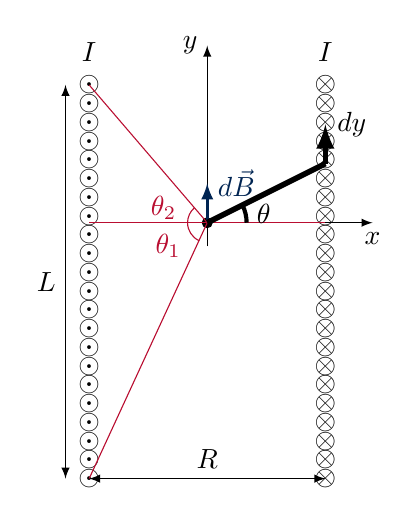
\begin{tikzpicture}[scale=1]

\tikzmath{
\R = 1.5;%charge radius
\f = 0.25;
\L = 5;
\Nt = 21;
\H=0.15*\L;
\Hy = 0.3*\L;
\dBl=0.5;
\t1 = atan( (\H+\L/2)/\R);
\t2 = atan( (\L/2-\H)/\R);
\t3 = atan( (\Hy-\H)/\R);
\dt = 0.25;
\dy=0.5;
}

%axes:
\draw[-latex] (0,\H-0.2*\R) -- (0,0.6*\L) node[left] {$y$};
\draw[-latex] (-0.2*\R,\H) -- (1.4*\R,\H) node[below] {$x$};

\foreach \i in {0,...,\Nt}{
 \tikzmath{
  \h = -\L/2+\i*\L/\Nt;
  }
 \node at (-\R,\h) {$\odot$};
 \node at (\R,\h) {$\otimes$};
 }

\coordinate (P) at (0,\H);
\fill (P) circle (2pt);
\draw[-latex, line width =1, color=qblue] (P) -- +(0,{\dBl}) node[right] {$d\vec B$};

\node[above=5pt] at (-\R,\L/2) {$I$};
\node[above=5pt] at (\R,\L/2) {$I$};


\draw[color=qred] (-\R,\H) -- (\R,\H);
\draw[color=qred] (P) -- (-\R,-\L/2);
\draw[color=qred] (P) -- (-\R,\L/2);

\draw[color=qred] (-\dt,\H) arc (180:180-\t2:\dt) node[left=3pt]{$\theta_2$} ;
\draw[color=qred] (-\dt,\H) arc (180:180+\t1:\dt) node[below=2pt,left=3pt]{$\theta_1$}; 

\draw[line width =2, -latex] (\R,\Hy) -- +(0,\dy) node[right]{$dy$};
\draw[line width =2] (P) -- (\R,\Hy);
\draw[line width =1.5] (2*\dt,\H) arc (0:\t3:{2*\dt}) node[midway,right] {$\theta$}; 

\draw[latex-latex] (-\R, -\L/2) -- (\R, -\L/2) node[midway,above] {$R$};
\draw[latex-latex] (-1.2*\R, -\L/2) -- (-1.2*\R, \L/2) node[midway,left] {$L$};

\end{tikzpicture}
\captionof*{figure}{\textit{Field inside of a solenoid}}
}



%%%%%%%%%%%%%%%%%%%%%%%%%%%%%%
\twocolframesf{Field inside of a solenoid using Ampère's Law}
{
\begin{itemize}
\item<1-> The field outside the solenoid is almost zero

\item<2> Using Ampère's Law, we have:
\only<2>{
\begin{align*}
\oint \vec B\cdot d\vec l &= Bl\\
I^{enc} &= NI\\
\therefore B &= \frac{\mu_0NI}{l}=\mu_0nI \quad \left(n=\frac{N}{L}  \right)
\end{align*}
}

\end{itemize}


}
{
\centering
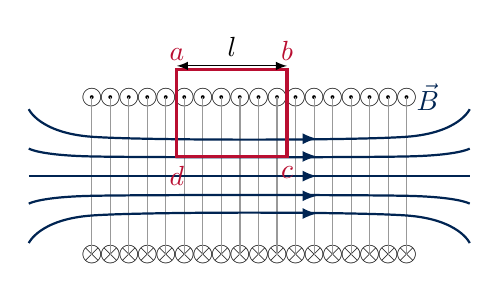
\begin{tikzpicture}[scale=1]

\tikzmath{
\R = 1;
\L = 4.0;
\Nt = 17;
\h=1;
\la=0.25*\R;
\LB=0.7*\L;
}
%
\foreach \i in {0,...,\Nt}{
 \tikzmath{
  \h = -\L/2+\i*\L/\Nt;
  }
  \node at (\h, \R ) {$\odot$};
  \node at (\h, -\R ) {$\otimes$};
  \draw[black!40] (\h, \R ) -- (\h, -\R );
}



%Field lines
%%midlle
\draw[color=qblue,thick] (-\LB,0) -- (\LB,0);

\draw[color=qblue,thick] plot [smooth,tension=0.5] coordinates {(-\LB,1.4*\la) (-0.5*\L,\la) (0.5*\L,\la) (\LB,1.4*\la)};
\draw[color=qblue,thick] plot [smooth,tension=0.5] coordinates {(-\LB,2*1.7*\la) (-0.5*\L,2*\la) (0.5*\L,2*\la) (\LB,2*1.7*\la)};
\draw[color=qblue,thick] plot [smooth,tension=0.5] coordinates {(-\LB,-1.4*\la) (-0.5*\L,-\la) (0.5*\L,-\la) (\LB,-1.4*\la)};
\draw[color=qblue,thick] plot [smooth,tension=0.5] coordinates {(-\LB,-2*1.7*\la) (-0.5*\L,-2*\la) (0.5*\L,-2*\la) (\LB,-2*1.7*\la)};


\draw[color=qblue,thick,-latex] (0.19*\L,0) -- +(0.1,0);
\draw[color=qblue,thick,-latex] (0.19*\L,\la) -- +(0.1,0);
\draw[color=qblue,thick,-latex] (0.19*\L,1.90*\la) -- +(0.1,0);
\draw[color=qblue,thick,-latex] (0.19*\L,-\la) -- +(0.1,0);
\draw[color=qblue,thick,-latex] (0.19*\L,-1.9*\la) -- +(0.1,0);

\node[color=qblue,right] at (\L/2,\R) {$\vec B$};

\coordinate (A) at (-0.23*\L,1.35*\R);
\coordinate (B) at (0.12*\L,1.35*\R);
\coordinate (C) at (0.12*\L,0.25*\R);
\coordinate (D) at (-0.23*\L,0.25*\R);

\draw[color=qred,very thick] (A) -- (B) -- (C) -- (D) -- cycle;
\node[color=qred, above] at (A) {$a$};
\node[color=qred, above] at (B) {$b$};
\node[color=qred, below] at (C) {$c$};
\node[color=qred, below] at (D) {$d$};

\draw[latex-latex] (-0.23*\L,1.4*\R) -- (0.12*\L,1.4*\R) node[midway,above] {$l$};

\end{tikzpicture}
\captionof*{figure}{\textit{Field inside of a solenoid}}
}



%%%%%%%%%%%%%%%%%%%%%%%%%%%%%%
\subsection{The toroid}
\label{subsec:thetoroid}
\twocolframesf{The toroid - a solenoid turned into a donut}
{
\begin{itemize}
\item This creates a magnetic field with circular field lines. 
\end{itemize}


}
{
\centering
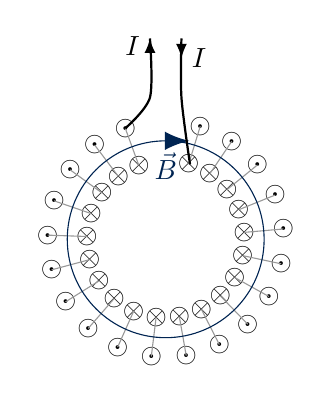
\begin{tikzpicture}[scale=1]

\tikzmath{
\Ri = 1;
\Ro = 1.5;
\Rb=0.5*\Ro+0.5*\Ri;
\Nt = 20;
\t1 = 10;
\t2 = 90-(360-2*\t1)/\Nt;
}
%
\foreach \i in {1,...,\Nt}{
 \tikzmath{
  \t = 90-\i*(360-2*\t1)/\Nt;
  }
  \node at (\t:\Ro) {$\odot$};
  \node at (\t:\Ri) {$\otimes$};
  \draw[black!40] (\t:\Ro)  -- (\t:\Ri) ;
}


\draw[color = qblue] (0,0) circle (\Rb);
\draw[color=qblue, line width =2pt,-latex] (0,\Rb) node[below] {$\vec B$} -- +(0.3,0) ;


\draw[black,thick] plot [smooth,tension=0.5] coordinates { (72:\Ri) (0.2,1.2*\Ro) (0.2,1.7*\Ro)};
\draw[black,thick] plot [smooth,tension=0.5] coordinates { (110:\Ro) (-0.2,1.2*\Ro) (-0.2,1.7*\Ro) };

\draw[-latex, thick] (0.2,1.6*\Ro) -- +(0,-0.1) node[right] {$I$};
\draw[latex-, thick] (-0.2,1.7*\Ro) -- +(0,-0.1) node[left] {$I$};

\end{tikzpicture}
\captionof*{figure}{\textit{A toroid.}}


}


%%%%%%%%%%%%%%%%%%%%%%%%




%%%%%%%%%%%%%%%%%%%%%%%%




%%%%%%%%%%%%%%%%%%%%%%%%




%%%%%%%%%%%%%%%%%%%%%%%





%%%%%%%%%%%%%%%%%%%%%%





%%%%%%%%%%%%%%%%%%%%%%%





%%%%%%%%%%%%%%%%%%%%%%







\end{document}